\documentclass[12pt]{article}

\usepackage{float}
\usepackage{fancyhdr}
\usepackage{amsmath}
\usepackage{amsthm}
\usepackage{mathrsfs}
\usepackage{graphicx}
\usepackage{graphics}
\usepackage{subcaption}
\usepackage{hyperref}
\usepackage{wrapfig}
\usepackage{arydshln}
\usepackage{multirow} 
\usepackage{tikz}

\usepackage[natbib=true,
    style=numeric,
    sorting=none]{biblatex}
\addbibresource{bibi.bib}

\begin{document}
\begin{titlepage}
	\centering
	{\textsc{University of Bonn} \par}
	\vspace{1cm}
	{\Large \textsc{Lab report}\par}
	\vspace{1.5cm}
	{\huge\bfseries High Resolution Laser Spectroscopy\par}
	\vspace{2cm}
	{\Large\itshape Wajdee Chayeb \\
	MohammadReza Torkamani\par}
	\vfill
	Tutors:\par
	Thilina Muthu-Arachchige\\
	Lukas Tenbrake

	\vfill

% Bottom of the page
	{\large \today\par}
\end{titlepage}

\tableofcontents


\section{Abstract}
The aim of this experiment is to study the characteristics of laser diodes and Fabry-Pérot interferometers using a diode laser optimized at a wavelength of 794 nm. This is done to perform linear spectroscopy to study Doppler-broadened transitions of Rubidium vapor. Then the spectral resolution is increased to eliminate the Doppler effect by performing non-linear spectroscopy. We verify the Lambert-Beer law and investigate the hyperfine structure, hyperfine coupling constants, and saturation intensity of Rubidium. In this report, we present the setup used, the analysis done, and the results obtained.

\section{Diode Laser Characteristics} 
Before performing spectroscopy, we investigate the properties of the used diode laser. This is done by measuring the dependence of the output power as a function of injection current to determine the threshold current, slope efficiency, and also the quantum efficiency. 

Figure \ref{fig1} illustrates the setup used for this part of the experiment. The laser beam is guided onto a photodiode to measure the output power. The beam is also attenuated such that for the maximum output power, the laser operates in the linear regime and not being saturated.  Laser emits a light of a wavelength of 794 nm \cite{lecturenote}.


\begin{figure}[H]
    \centering
    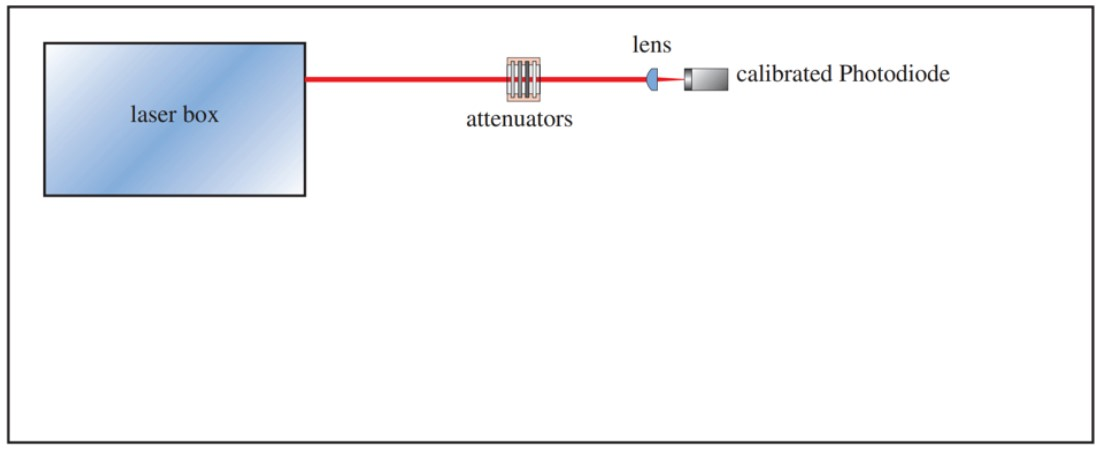
\includegraphics[width = \textwidth]{fig/setup1.jpg}
    \caption{Schematic view of the setup used for leaser output power measurement\cite{lecturenote}}
    \label{fig1}
\end{figure}

We show in Figure \ref{fig2}, the dependence of laser output power on the obtained injection current. To account for measurement errors, we choose the highest varying digit of the measuring device. Here, we see that prior to a certain value of the injection current, the output power remains constant, a behavior similar to light-emitting diodes (LED) \cite{led}. However, beyond the threshold current,  ($54 \pm 1 \mathrm{mA}$), a kink in the output power is realized and the correlation becomes linear. To quantify this linear behavior, we fit a linear function using the Python script $optimize.curve\_fit$ \cite{scipy}.  From the fit, we get a slope efficiency of:

\begin{equation*}
    \frac{\delta P_{out}}{\delta I} 
    = (10.41 \pm 0.08) \frac{mW}{mA} 
\end{equation*}


\begin{figure}[H]
    \centering
    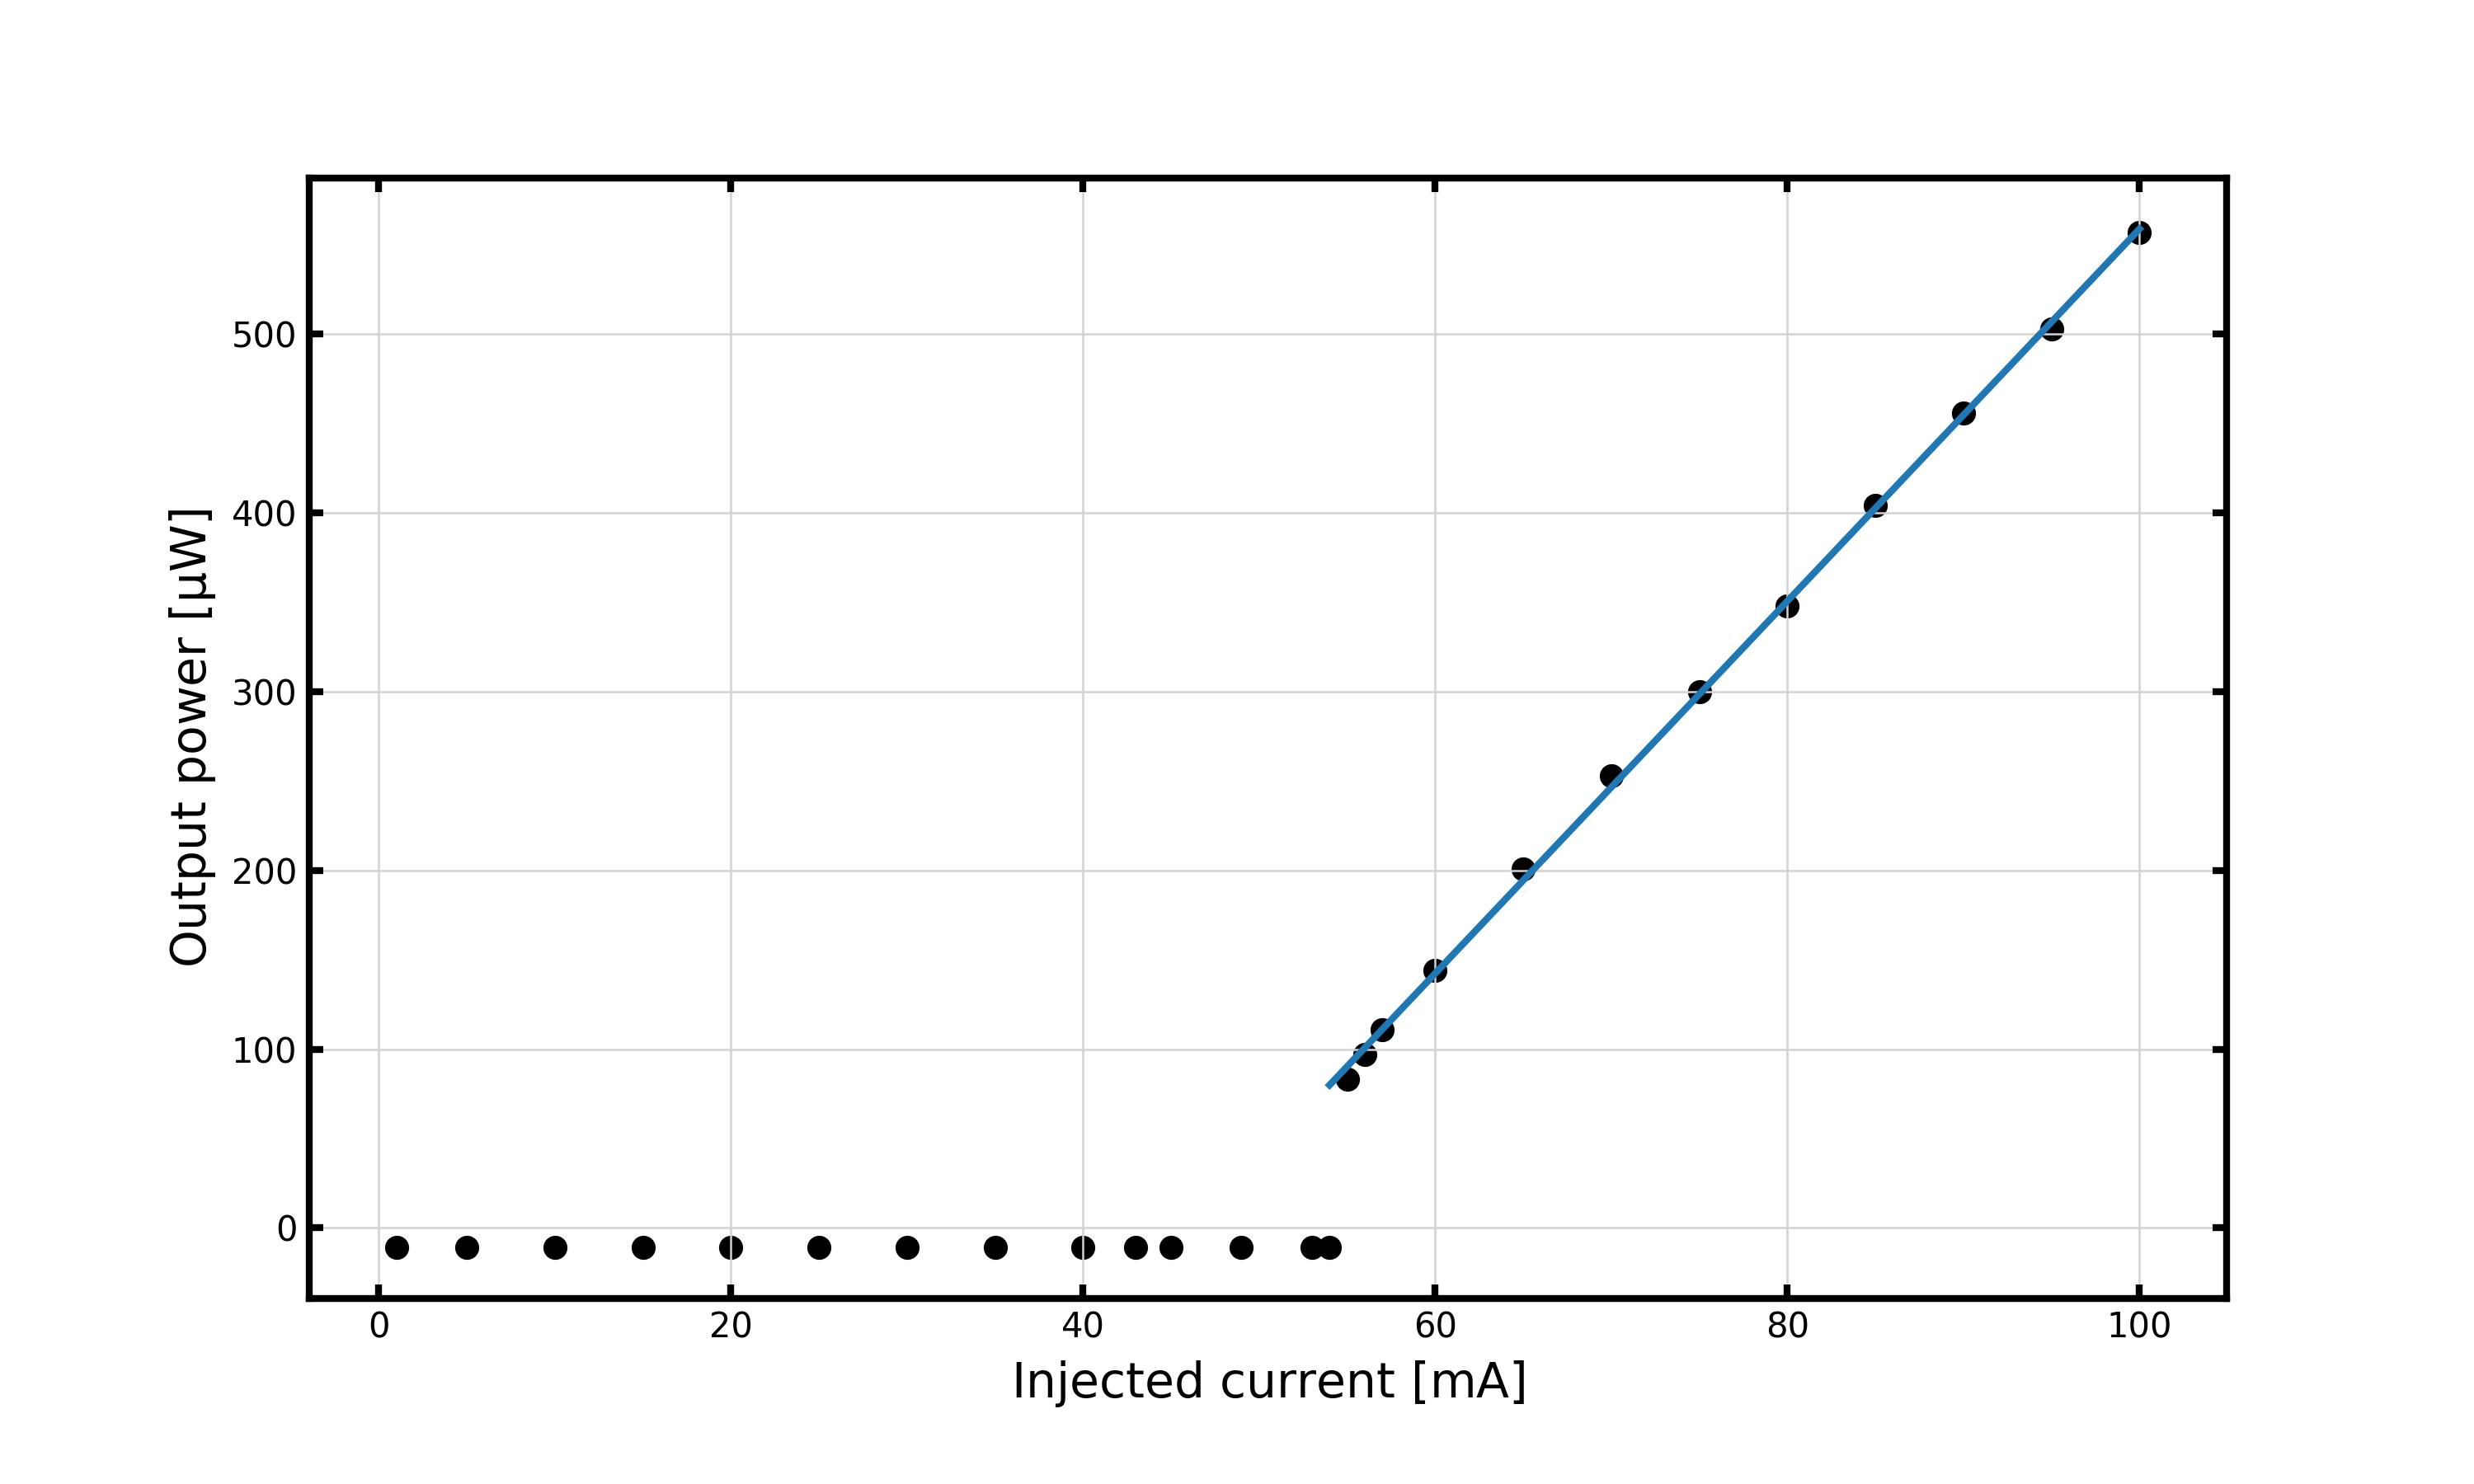
\includegraphics[width = \textwidth]{fig/Laserchar.png}
    \caption{Dependence of laser output power on injection current}
    \label{fig2}
\end{figure}

Moreover, we calculate the quantum efficiency $\eta$, number of emitted photon per injected electron, as \cite{lecturenote}:

\begin{equation}
    \eta = \frac{N_{\gamma}/t}{N_{e}/t} = \frac{P/E(\lambda = 749 nm)}{I/e}
    \label{eq1}
\end{equation}

Where $N_{\gamma}$ is the number of emitted photons, $N_{\gamma}$ is the number of electrons, P is the power, E is the energy of one photon emitted at the laser frequency, and e is the value of electron charge. We present the results of the dependence of quantum efficiency on the injected current in Figure \ref{fig3}. As seen from the figure, An increase in the efficiency for increasing current is recognized. However, the increase is small. 

\begin{figure}[H]
    \centering
    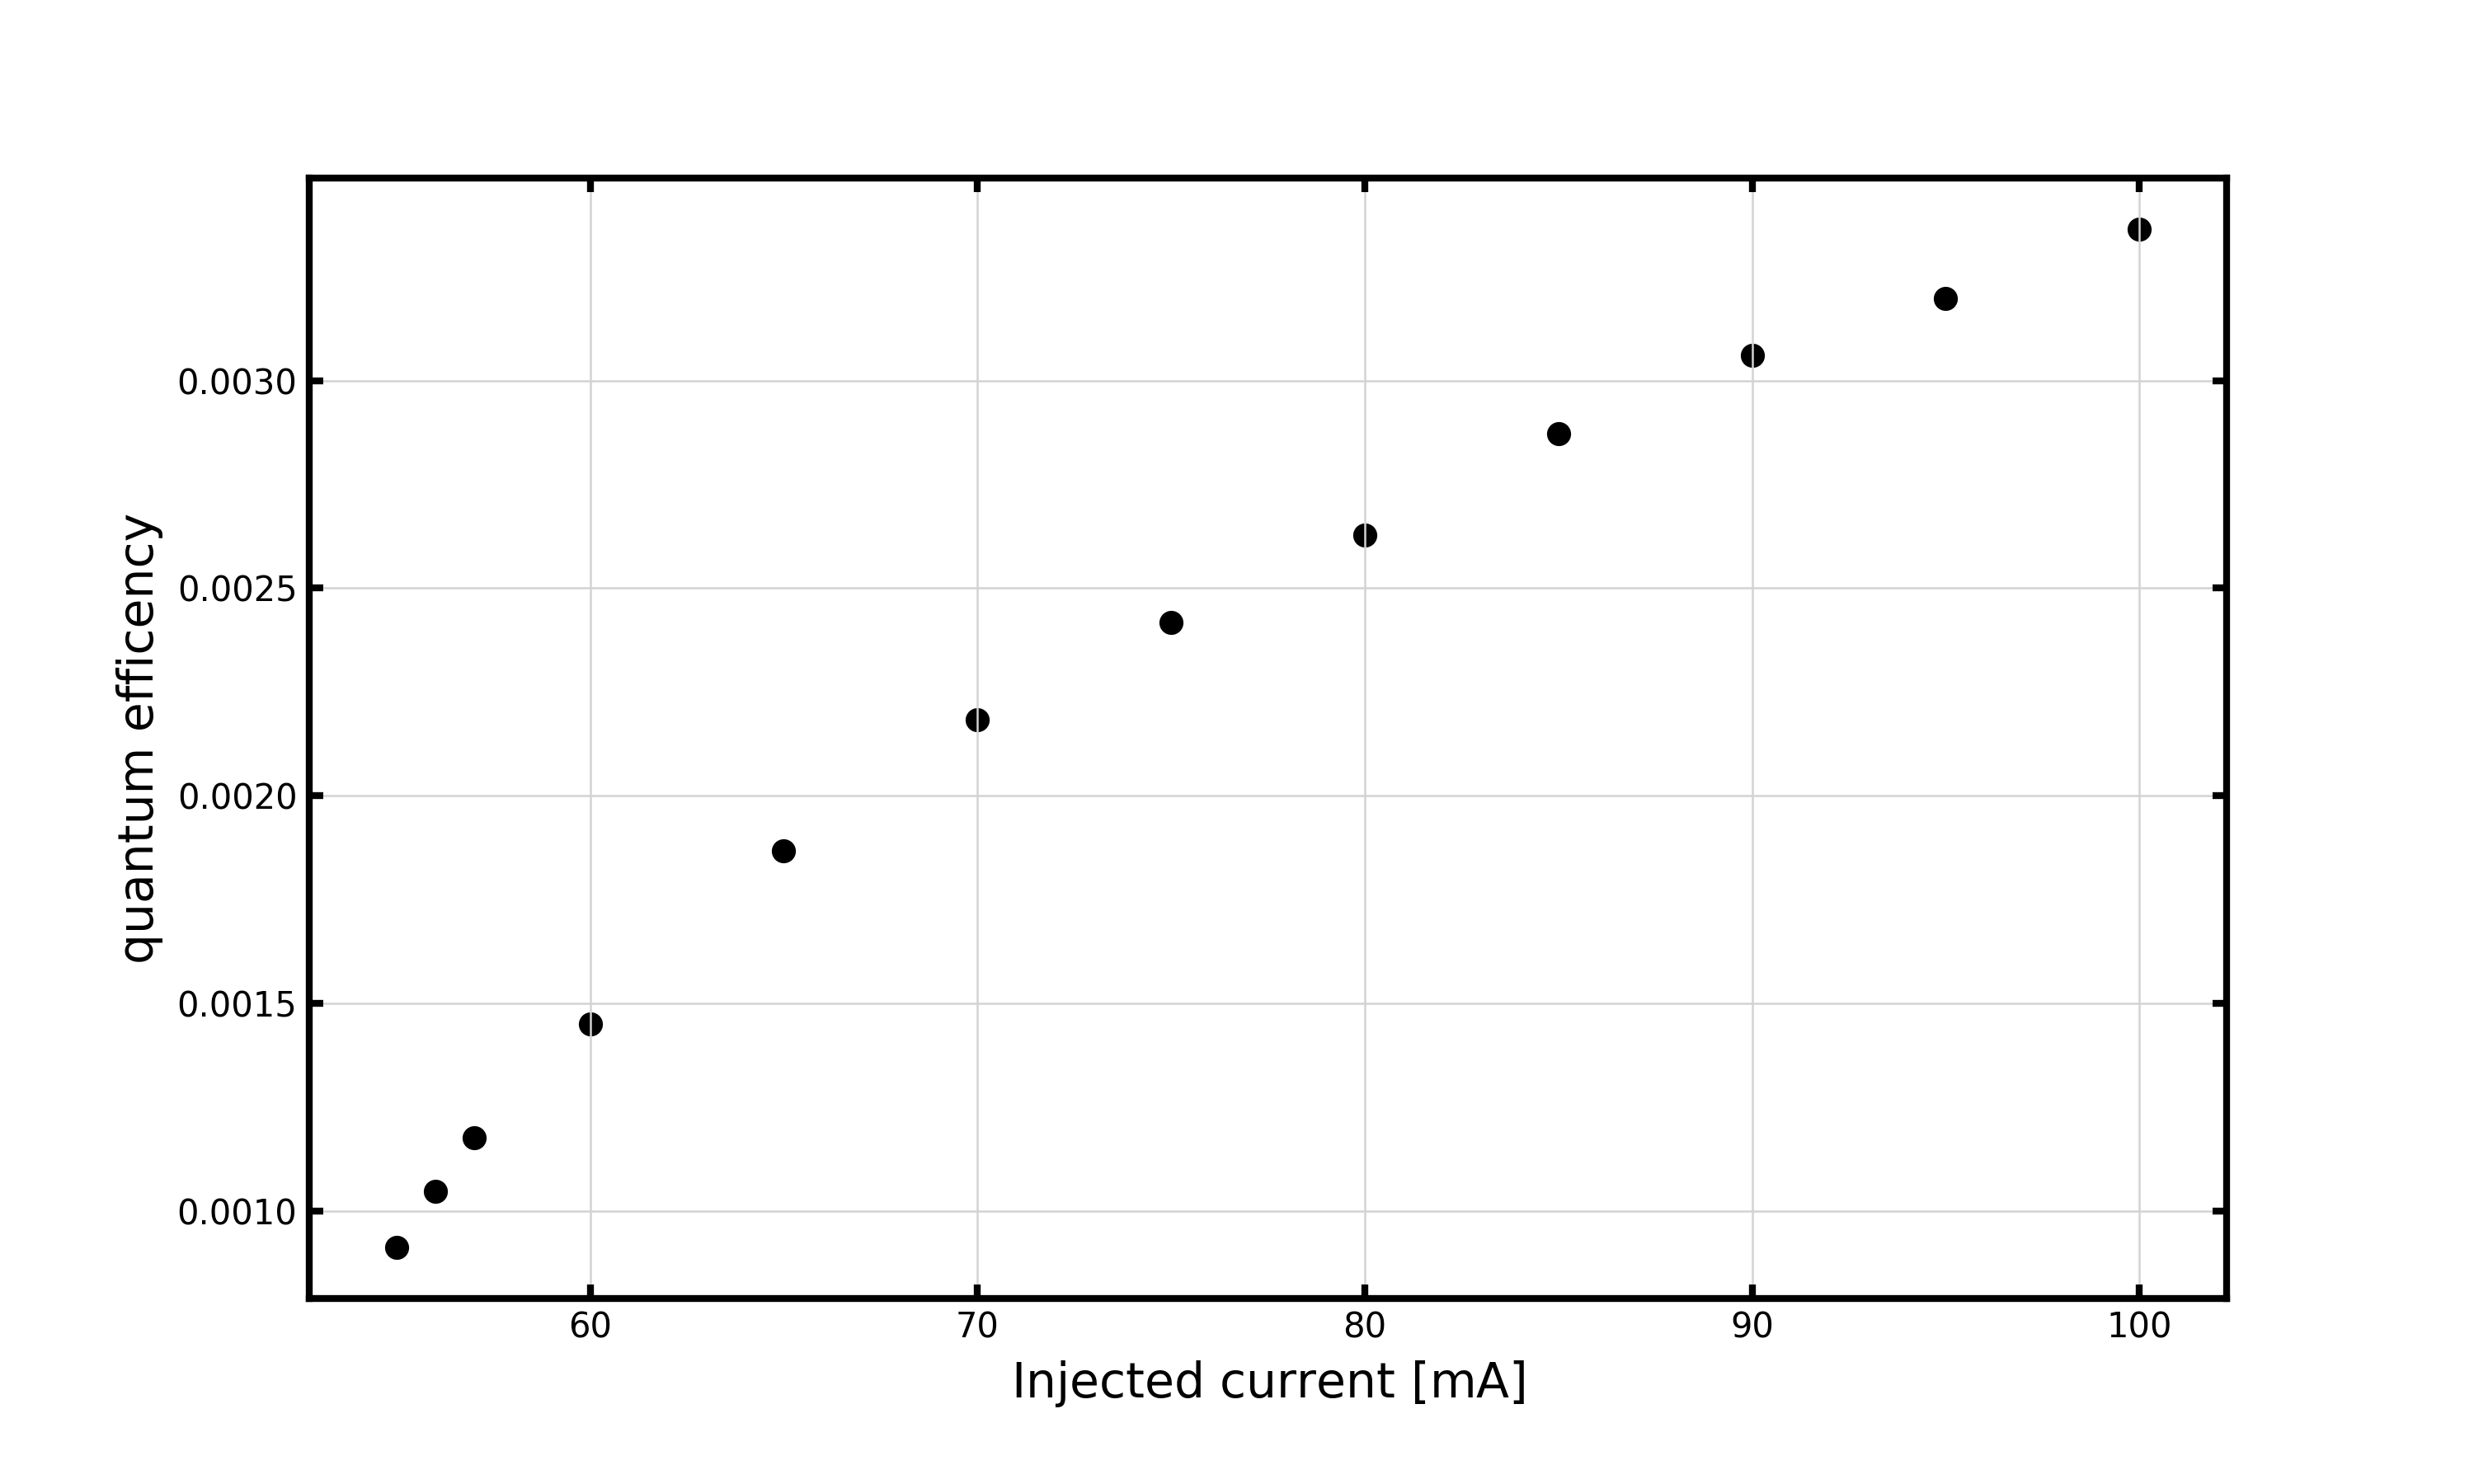
\includegraphics[width = \textwidth]{fig/Quantum_efficency.png}
    \caption{Dependence of quantum efficiency on the injection current}
    \label{fig3}
\end{figure}


% and $I_{thr}$ = $\pm$

% fiting parameters
% slope = 10.41 ± 0.08
% intercept = -482.2 ± 6.2

\section{Use of The Fabry-Pérot Interferometer}

We use a Fabry-Pérot Interferometer (FPI) to set a reference to convert the oscilloscope's measurements of the tile elapsed during the scan of the Rubidium spectrum to relative frequencies. This allows us to calculate relative energy shifts of the hyperfine transition levels and also the hyperfine coupling constants. 
We start by investigating the properties of the FPI such as its finesse and establishing a conversion method for arbitrary time units to frequencies.   

Since the spectrum of SPI shows peaks in uniform frequency intervals, a frequency calibration is possible, and the transmission is expressed as \cite{lecturenote}:
\begin{equation}
    T_{FPI} = \frac{1}{1 + F sin^{2}(\phi/2)}
    \label{eq2}
\end{equation}

Where $T_{FPI}$ is the transmission of the FPI, F is a coefficient that describes the finesse, and $\phi$ is a relative phase shift a light accretes in the FPI. This shift is also expressed as \cite{lecturenote}:

\begin{equation}
    \frac{\phi}{2} = \frac{2 \pi n \nu L}{c}
    \label{eq3}
\end{equation}
Where n is the refractive index of the FPI, $\nu$ is the frequency of light used, L is the length of the FPI, and c is the speed of light.

the finesse of the FPI is given as \cite{lecturenote}:
\begin{equation}
    \mathcal{F}=\frac{\pi \sqrt{F}}{2}=\frac{\pi \sqrt{R}}{1-R}
    \label{eq4}
\end{equation}
R here is the reflectivity of the used mirrors.
When conducting the measurement, first the the finesse is measured and then a conversion of elapsed time to relative frequencies is done. The finesse for a perfect FPI with only losses occurring at the reflecting mirrors is calculated as \cite{lecturenote}:
\begin{equation}
    F=\frac{4 R}{(1-R)^2}
    \label{eq5}
\end{equation}

Using eq. \ref{eq4}, we calculate the finesse for a mirror reflectivity R = 0.85. We get $\mathcal{F}$ = 19.31. 
Then, we find a relation between the full-width half maximum (FWHM) frequency $\delta \nu_{FWHM}$ of the transmission peaks and the frequency intervals between the peaks, which is characterized by the free spectral range $\Delta \nu_{FSR}$. This is done by using eq. \ref{eq2}. 
If the FPI achieves a high finesse, the transmission outside the peaks approaches zero and we get:
\begin{equation}
    T_{\mathrm{FPI}}\left(\nu_0+\frac{\delta \nu_{\mathrm{FWHM}}}{2}\right)=\frac{1}{2} T_{\mathrm{FPI}}\left(\nu_0\right)  
    \label{eq6}
\end{equation}

Where $\nu_0$ is the frequency at the peak of transmission. 
For $\phi/2 = m\pi$, we have $T_{\mathrm{FPI(\nu_0)}}$ = 1. This occurs at frequencies of $\nu_0 = \frac{mc}{2nL}$. Then, a frequency interval between two peaks $\Delta \nu_{FSR}$ can be expressed as"
\begin{equation}
    \Delta \nu_{FSR} = \frac{c}{2nL}
    \label{eq7}
\end{equation}
For rearrangement of eq. \ref{eq6}, we get: 
\begin{equation}
    F \sin ^2\left(2 \pi n\left(\nu_0+\frac{\delta \nu_{\mathrm{FWHM}}}{2}\right) \frac{L}{c}\right)=1
    \label{eq8}
\end{equation}

By Taylor expanding eq. \ref{eq8} around
$2 \pi n \nu_0 \frac{L}{c}$, we get:
\begin{equation}
    F\left(\pi n \delta \nu_{\mathrm{FWHM}} \frac{L}{c}\right)^2=1
    \label{eq9}
\end{equation}
Using \ref{eq9}, solving for  $\delta \nu_{\mathrm{FWHM}}$ yields:

\begin{equation}
    \delta \nu_{\mathrm{FWHM}}=\frac{2}{\pi \sqrt{F}} \Delta \nu_{\mathrm{FSR}}=\frac{\Delta \nu_{\mathrm{FSR}}}{\mathcal{F}}
    \label{eq10}
\end{equation}

\subsection{Experimental Setup}
Figure \ref{fig4} illustrates the experimental setup used for measuring the transmission of the laser through the FPI. A wedge is placed into the beam acting as a beam splitter to divide the beam, so we get there laser beams, a strong one and two weaker beams that are diffracted or reflected, to be used in further steps. For this part, two of the beams are blocked and only one of the weaker beams is used to measure the FPI spectrum.  
The beam used is guided to pass through a pinhole to backscattering minimization from the FPI and then coupled into the FPI using the two mirrors. The incoming beam has to be parallel to the FPI so it does not get reflected from the side wall of the FPI. Since the laser wavelength is in the infrared regime, we use a fluorescing viewing card to track the trajectory of the beam. 
Then, a focusing lens is used to focus the beam on a photodiode, which measures the incoming power and is monitored with an oscilloscope. 
To tune the laser frequency periodically, we vary the tilting of an echelette grating in Lithrow configuration using a piezoelectric transducer (PZT). Since there is no absolute frequency, the setup only provides a relative calibration with respect to an arbitrary zero frequency.

\begin{figure}[H]
    \centering
    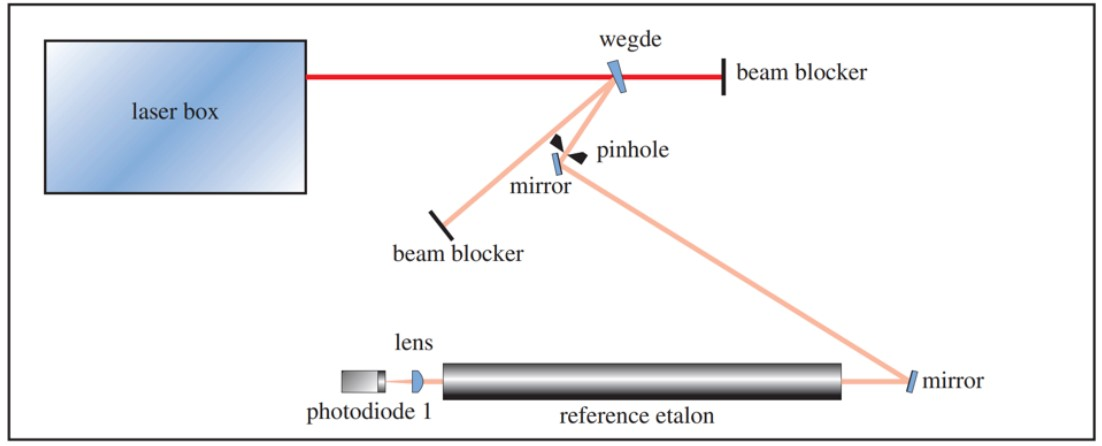
\includegraphics[width = \textwidth]{fig/setup2.jpg}
    \caption{Experimental setup used for measuring the transmission of the laser through the FPI \cite{lecturenote}}
    \label{fig4}
\end{figure}

\subsection{Finesse Measurement}

\begin{figure}[H]
    \centering
    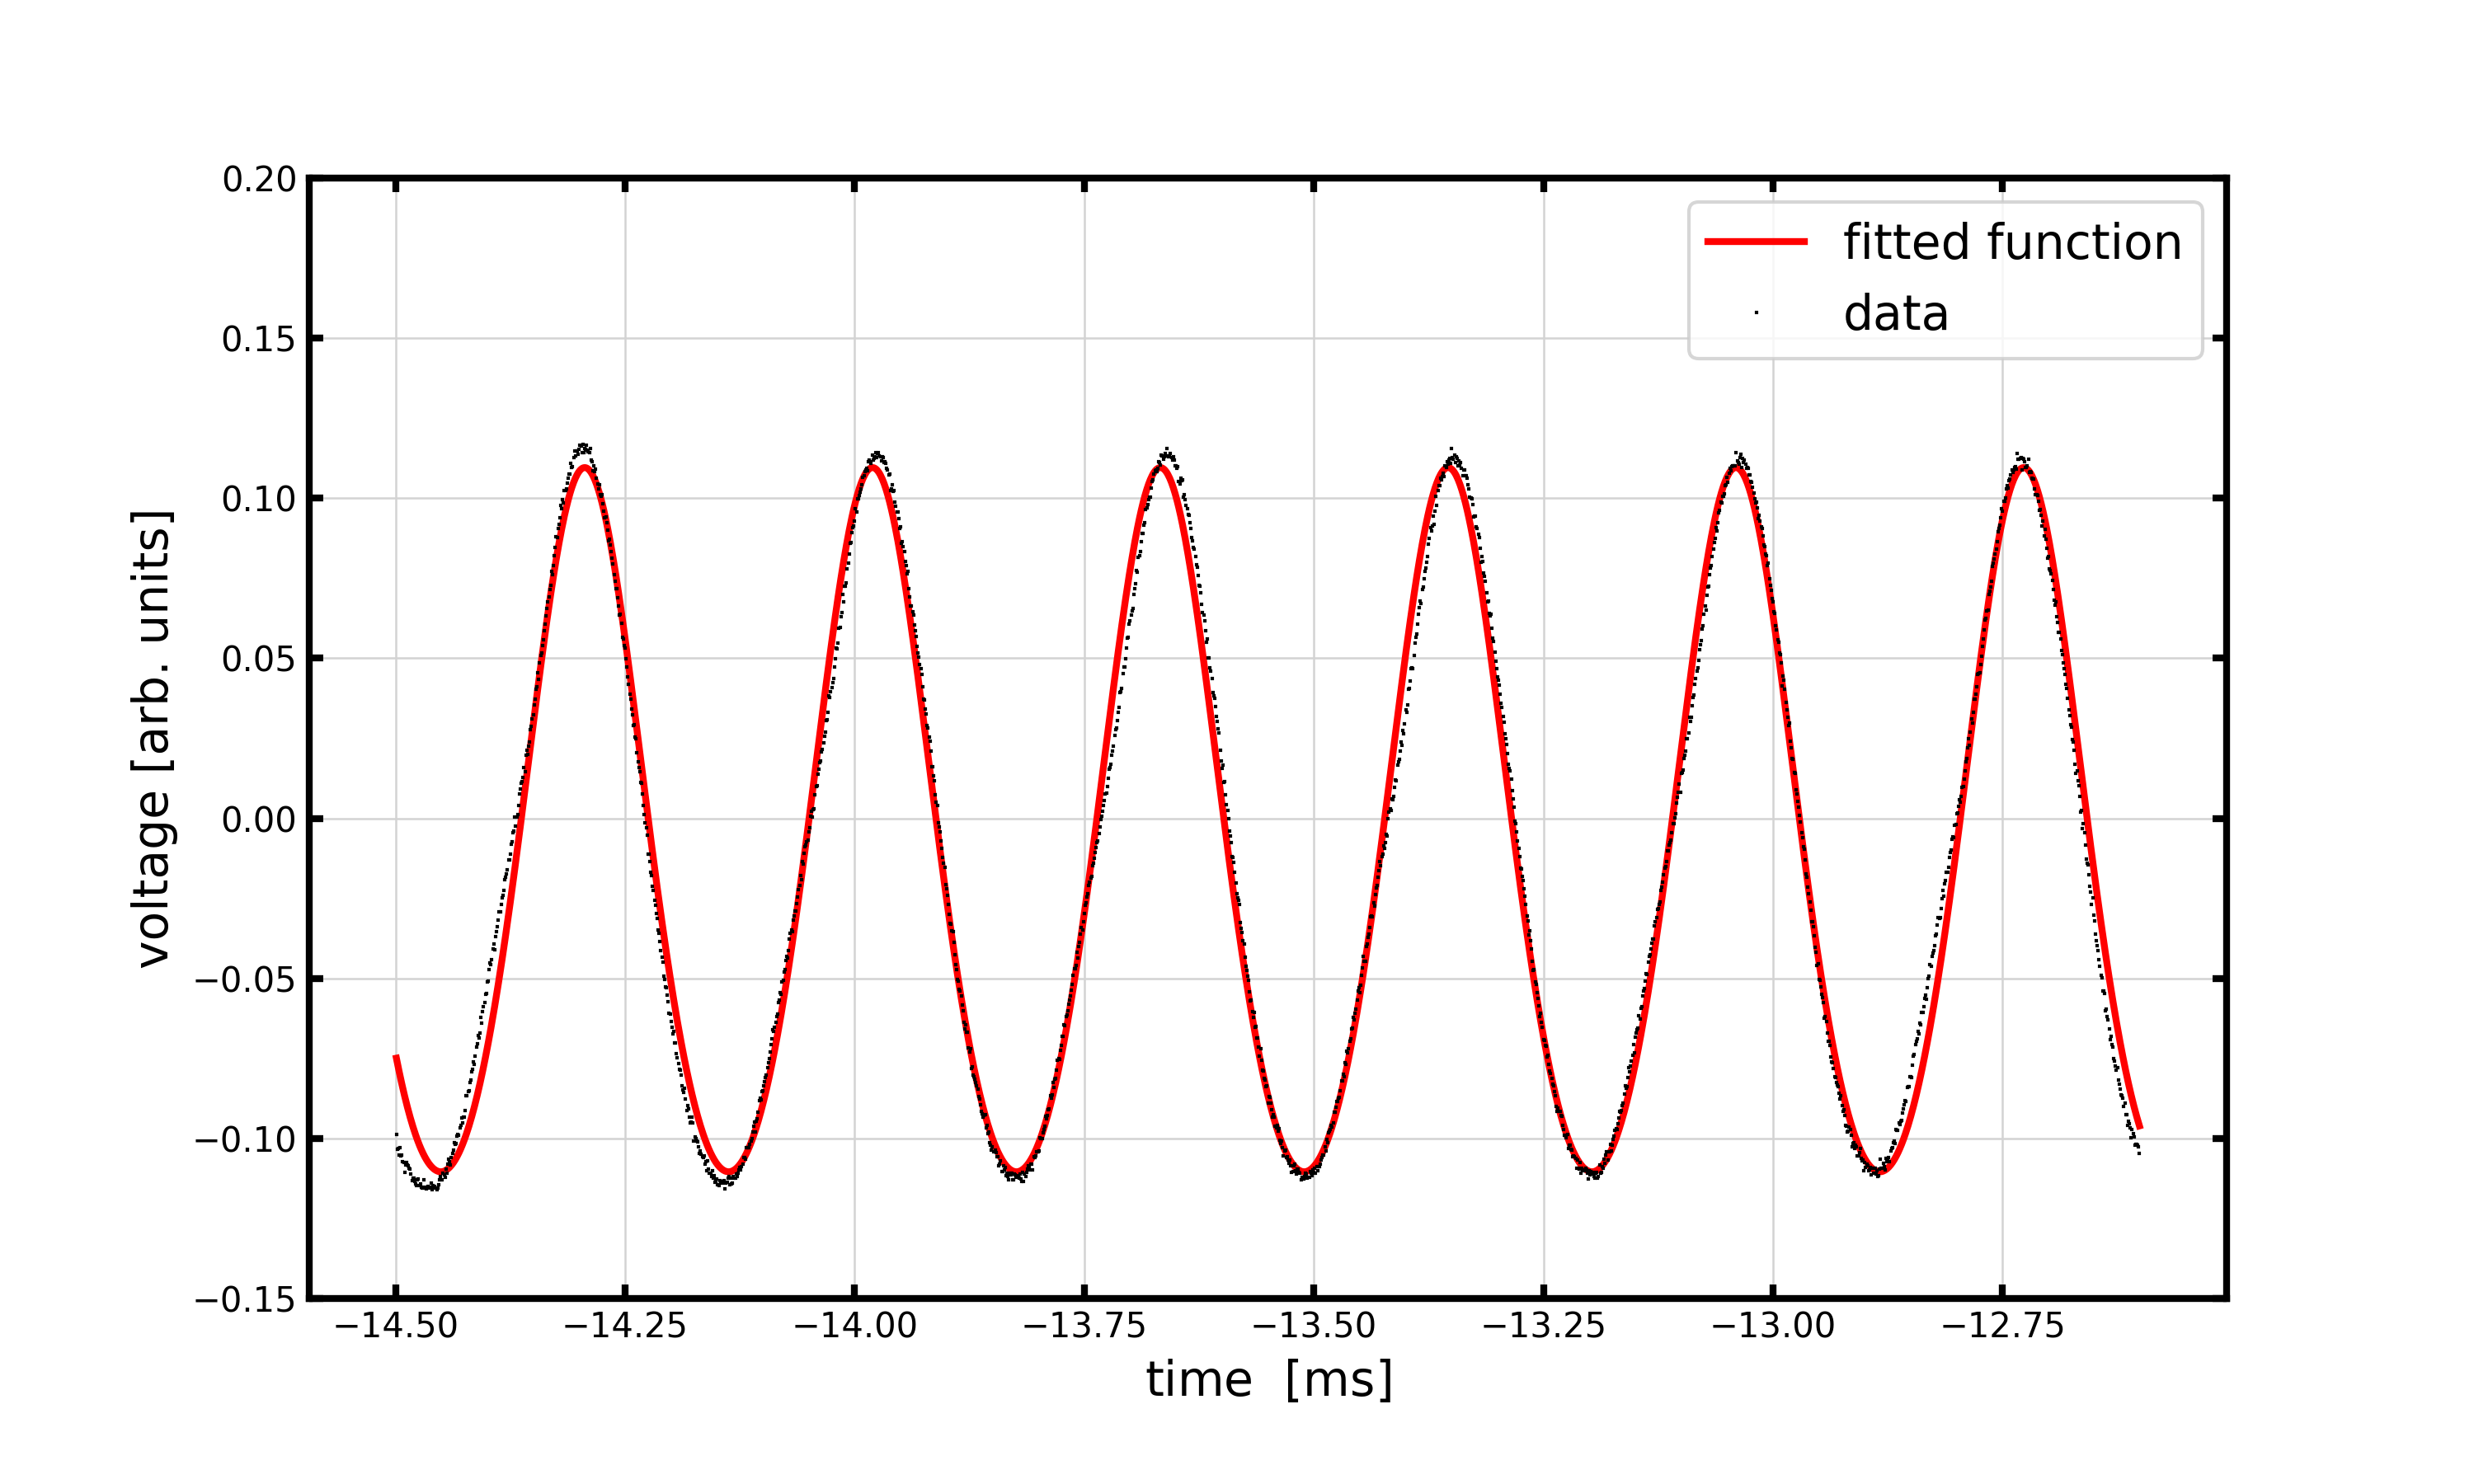
\includegraphics[width = \textwidth]{fig/FPI.png}
    \caption{Transmission spectrum of the FPI}
    \label{fig5}
\end{figure}

Figure \ref{fig5} displays the transmission spectrum of the FPI. We start by applying a fit to the spectrum using a function of a form similar to \ref{eq2}, expressed as:
\begin{equation*}
    y=\frac{a}{1+b \sin ^2(c t+d)}+e    
\end{equation*}
The fit provides a good description of the data (black curve in Figure \ref{fig5}), except for the peaks. All fitting parameters are reported in Table \ref{tab1}.

\begin{table}[H]
    \centering
    \begin{tabular}{c|c|c|c|c}
         \hline
         \hline
         a & b & c & d & e  \\
         \hline
         $0.715 \pm 0.02$ & $0.445 \pm 0.015$ & $10024.986 \pm 2.331$ & $14.491 \pm 0.032$ & $-0.605 \pm 0.017$\\
         \hline
    \end{tabular}
    \caption{Fitting parameters of the fitting spectrum of the FPI}
    \label{tab1}
\end{table}

eq. \ref{eq10} is used to calculate the finesse. $\mathcal{F}$ can be calculated without calibration using $\delta t_{FWHM}$ and $t_{SFR}$ since both $\delta\nu_{FWHM}$ and $\nu_{SFR}$ have linear dependence on them with the same proportionality. 
As a result, $\delta t_{FWHM}$ is calculate as:
\begin{equation*}
    \delta t_{FWHM} = \frac{2}{\sqrt{b}c} = 0.299 \pm 0.005 \mathrm{ms}
\end{equation*}
Due to the interplay between transverse and longitudinal modes, the distance between two peaks with a peak between them is used to calculate $t_{SFR}$ as:
\begin{equation*}
    t_{SFR} = \frac{2\pi}{c} = 0.6248 \pm 0.0003 \mathrm{ms}
\end{equation*}

Now using, eq. \ref{eq10}, we get: 
\begin{equation*}
    \mathcal{F} = \frac{\Delta \nu_{\mathrm{FSR}}}{\delta \nu_{\mathrm{FWHM}}} = 2.08 \pm 0.03 
    \label{eq100}
\end{equation*}

The resulting value deviates from the theoretical calculation of 19.31. This strong deviation is possible due to multiple reasons. First, impurities on the surface of the mirrors of the FPI (e.g. scratches) can cause the deviation. Second, the reflectivity of the mirrors used is R = 0.59, but not the assumed value of R = 0.85. Third, a distortion of the mirrors or any misalignments in the setup. One has also to account for the error resulting from the oscilloscope and readings. 

\subsection{Frequency Calibration}
The mode spacing is given as \cite{lecturenote}:
\begin{equation}
    \Delta \nu_{mode} = (149.9348 \pm 0.0002) MHz 
    \label{eq11}
\end{equation}
Since the firing spacing is almost constant, a linear function is used to calibrate the frequencies. The fringe spacing in time is given by:
\begin{equation}
    t_{mode} = \frac{t_{SFR}}{2} = 0.3124 \pm 0.0002\pm \mathrm{ms}
    \label{eq12}
\end{equation}
Thus, the calibration constant is:
\begin{equation*}
    c_{calibration} = (479.94 \pm 0.242) \mathrm{MHz /ms}
\end{equation*}

\section{Linear Spectroscopy}
In this part of the experiment, we investigate the hyperfine structure of $^{85}Rb$ and $^{87}Rb$ using linear spectroscopy. We determine the main characteristics of the hyperfine structures such as the hyperfine constants, examine the spectral resolution, and also compare the obtained FWHM of the transition lines to the expected value given by Doppler broadening. Furthermore, we verify the Lambert-Beer law by measuring the transmission through rubidium vapor cells with different lengths. 

\subsection{Hyperfine Splitting}
The total angular momentum of an atomic state is expressed as \cite{lecturenote}:
\begin{equation*}
    \vec{F}=\vec{I}+\vec{J}
\end{equation*}
Where $\vec{I}$ is the angular momentum of the nucleus (I = 5/2 for $^{85}Rb$ and I = 3/2 for $^{87}Rb$) and $\vec{J}$ is the angular momentum of the electron ($\vec{J}$ = 1/2 in the studied states).

The possible quantum states for $F$ are $|I-J| \leq F \leq I+J$, therefore the possible quantum states for ${ }^{85} \mathrm{Rb}$ are $F=2,3$ and for ${ }^{87} \mathrm{Rb}$ are $\bar{F}=1,2$.

The Hamiltonian for the hyperfine structure expressed as
$$
\hat{\mathcal{H}}_{\mathrm{hfs}}=A_{\mathrm{hfs}}\left(n L_j\right) \vec{I} \cdot \vec{J}
$$

which is also expressed as:
\begin{equation}
    \hat{\mathcal{H}}_{\mathrm{hfs}}=E_{\mathrm{hfs}}=A_{\mathrm{hfs}}\left(n L_j\right) \frac{1}{2}(F(F+1)-I(I+1)-J(J+1))
    \label{hyperfine}
\end{equation}

As the hyperfine coupling constant is positive, the higher quantum number $F$ corresponds to higher energies in the term diagram in Figure \ref{fig6}. Therefore, $F_{\mathrm{b}}=3, F_{\mathrm{a}}=2, F_{\mathrm{c}}=1$ and $F_{\mathrm{d}}=2$.

Using eq.\ref{hyperfine}, the following table containing the energy shifts can be obtained:
\\


\begin{figure}[H]
    \centering
    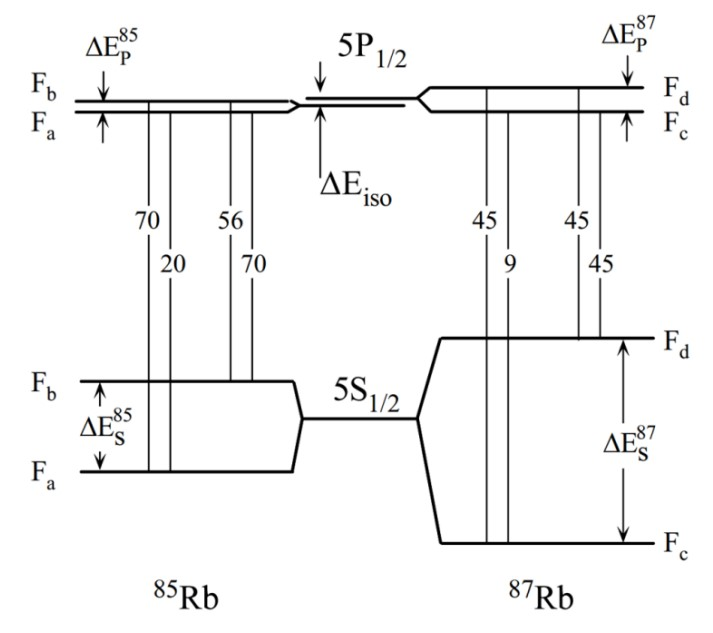
\includegraphics[width = \textwidth]{fig/Term diagram.jpg}
    \caption{Term diagram of Experimental Setup $^{85}Rb$ and $^{87}Rb$ \cite{lecturenote}}
    \label{fig6}
\end{figure}

\subsection{Expected Theoretical Absorption Spectrum}

By utilizing the level diagram \ref{fig6} and incorporating the calculated energy shifts for hyperfine structure, along with the relative transition probabilities, it is possible to derive a theoretically predicted absorption spectrum. In order to accomplish this, we start by obtaining the transition frequencies associated with the fine structure. These transition frequencies are as follows: $\nu = 377.107 385 690 \times 10^{12}$Hz and $\nu = 377.107 463 5 \times 10^{12}$Hz for $^{85}Rb$ and $^{87}Rb$ respectively \cite{Rb85}\cite{Rb87}.

We calculate the transition frequencies of each hyperfine level by first assuming a temperature of 300K, and that each line has a Gaussian shape since we expect them to be Doppler broadened. We account for the isotopic shifts and also get the atomic masses of Rubidium from \cite{Rb85}\cite{Rb87}. The depths of the absorption peaks, measured in relation to complete transmission of 100\%, are extracted from the term diagram \ref{fig6}. The hyperfine energies are added to the fine structure energy, increasing or reducing the frequency depending on the sign. 

After comparing the transition probabilities in Figure \ref{fig6} with the amplitude of each peak, we scale the amplitudes of the isotopes according to their occurrence in the vapor cell, where $^{85}Rb$ is 72.17\% of the total gas and $^{87}Rb$ represent 27.83 \% of the gas. 
The expected spectrum is shown in Figure \ref{fig7}. As seen from the figure, the lines of the measured spectra can be clearly identified. However, the hyperfine splitting of the excited state of $^{85}Rb$ is not resolved due to Doppler broadening of the lines, which is expected from linear spectroscopy. Thus, the need for linear spectroscopy to resolve these lines is inevitable. 

\begin{figure}[H]
    \centering
    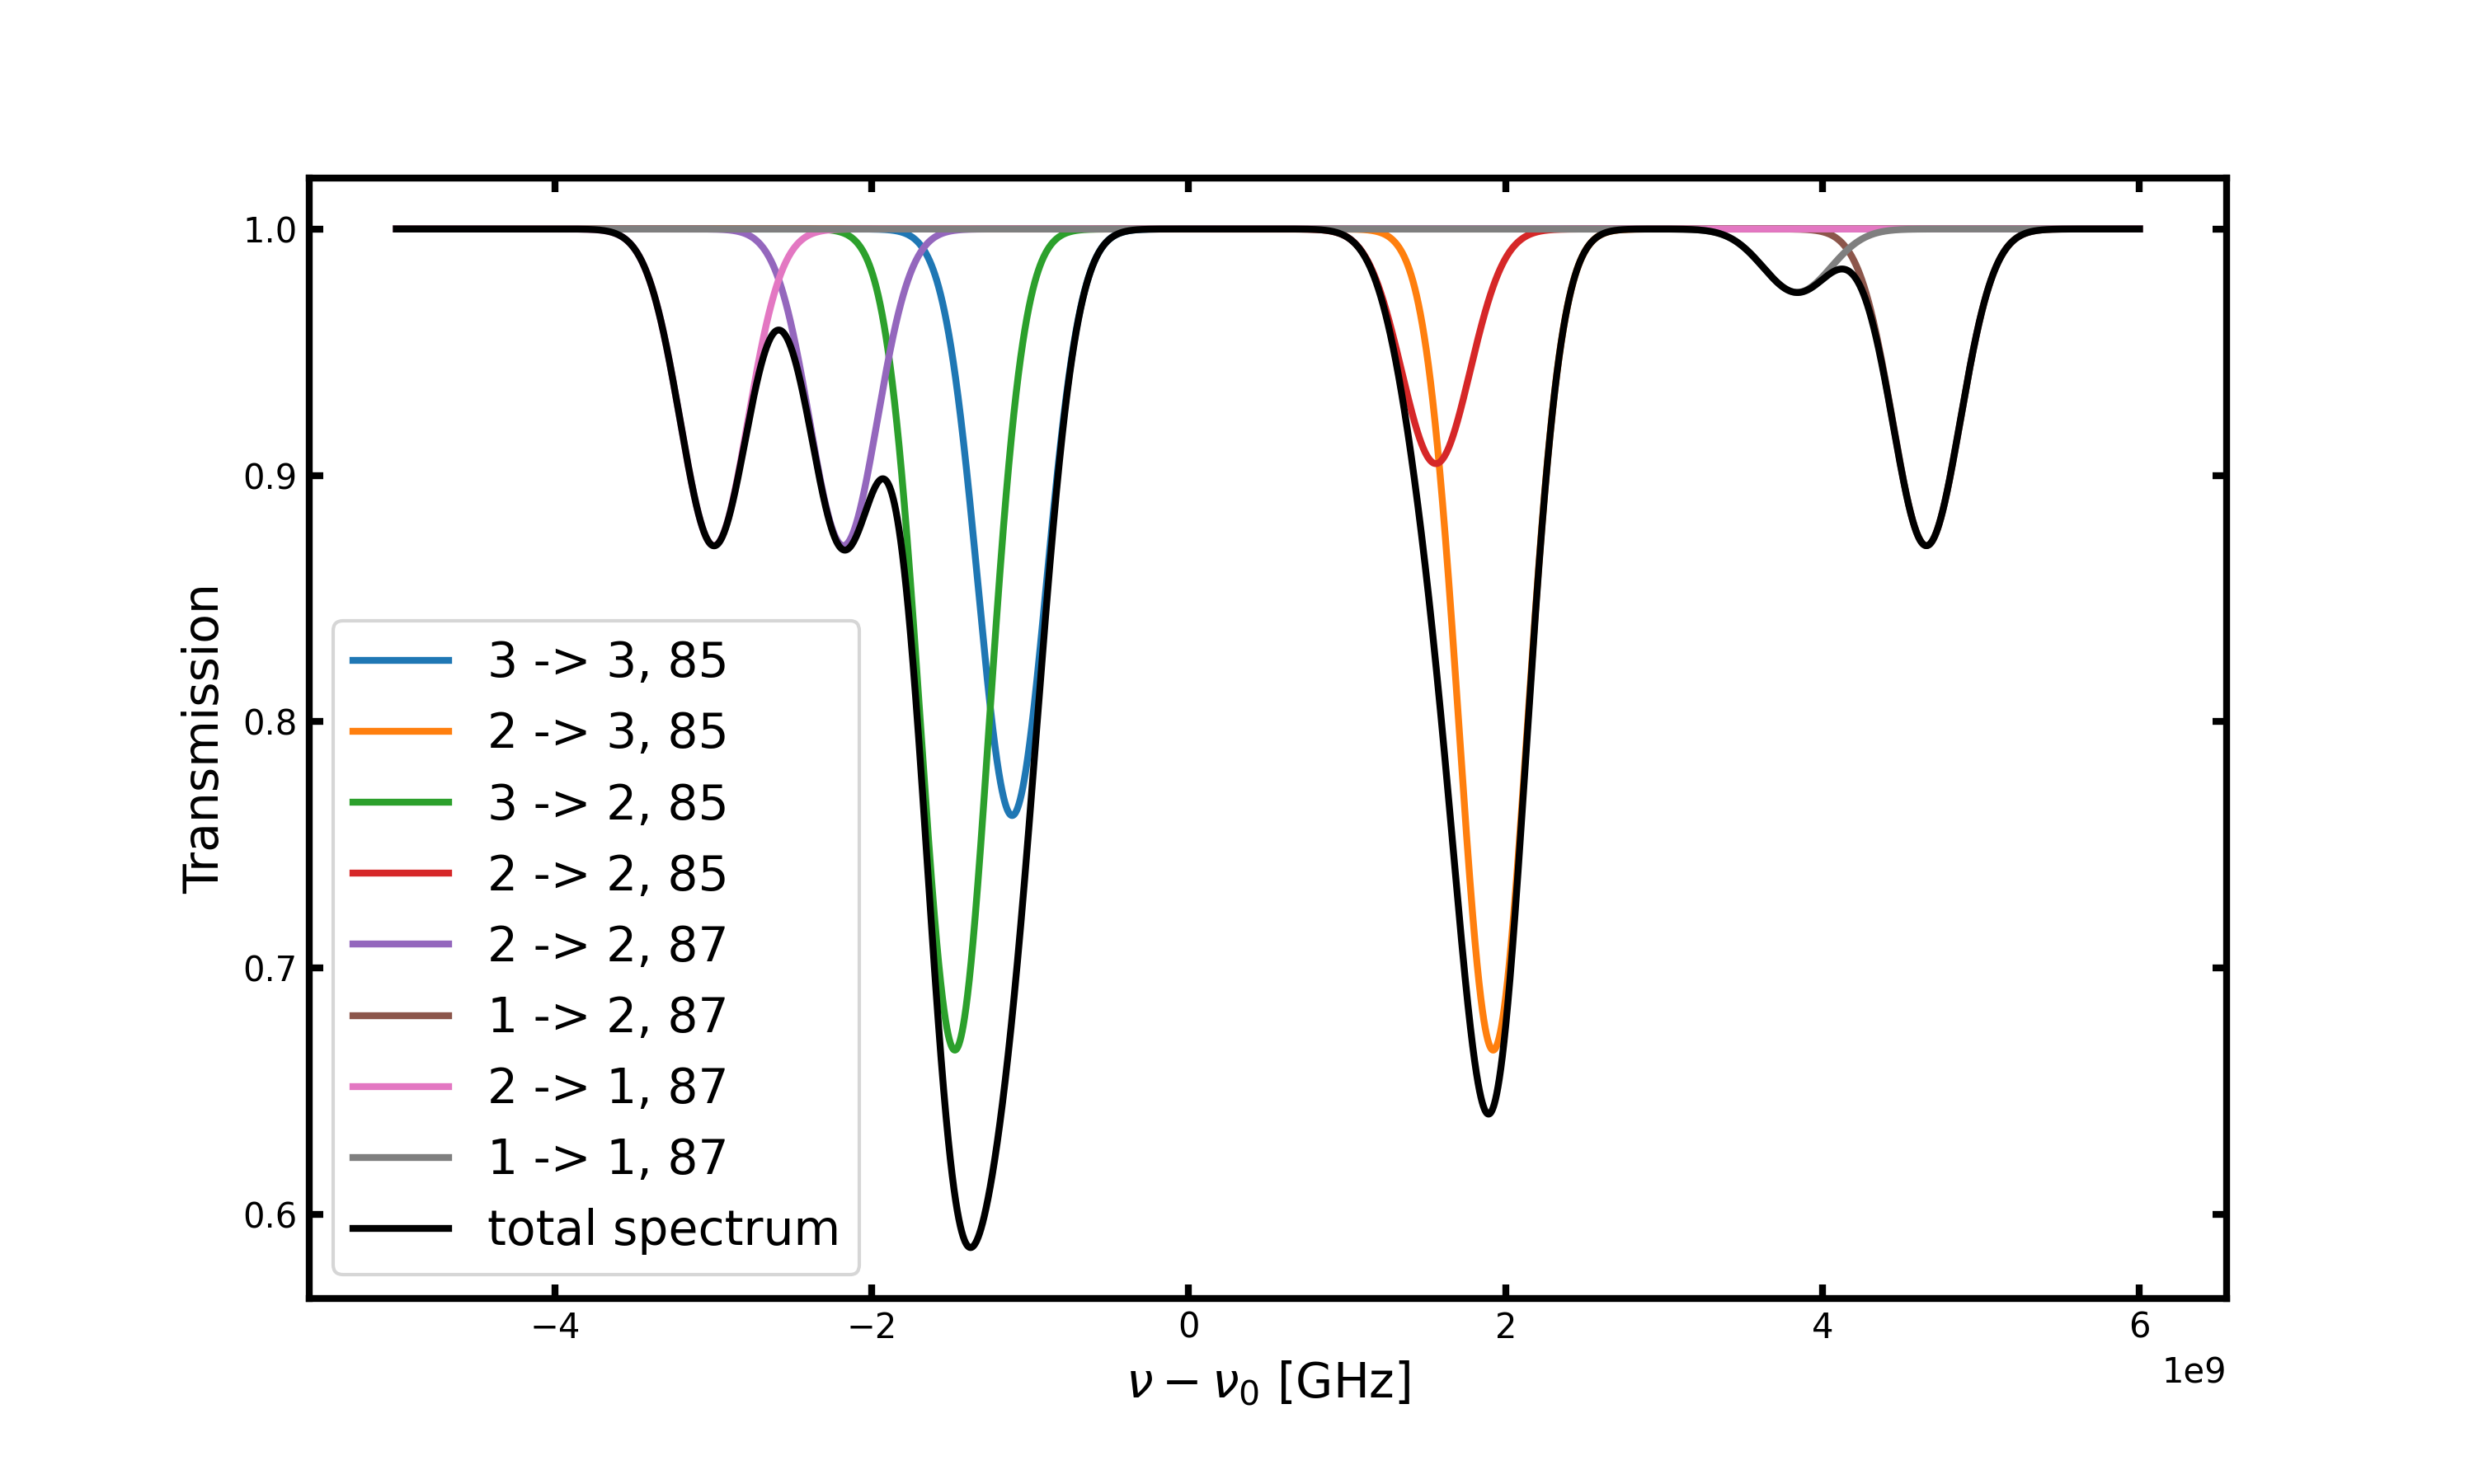
\includegraphics[width = \textwidth]{fig/Theoretical_spectrum.png}
    \caption{Expected theoretical absorption spectrum of $^{85}Rb$ and $^{87}Rb$}
    \label{fig7}
\end{figure}


\subsection{Experimental Setup}
Figure \ref{fig8} shows the experimental setup used for the part of linear spectroscopy in this experiment.  We use the same beam transmitted through the wedge in the previous section \ref{fig4} and remove the beam blocker. The beam is attenuated to decrease the intensity to around 20 $\mu$W and guided by two mirrors to be pointed into the Rb vapor cell of 5 cm length.  Again, to measure the power, we focus the beam on a photodiode whose
measurement is monitored on the oscilloscope along with the transmission through the FPI, this is done to ensure that the laser runs in a single mode. 
\begin{figure}[H]
    \centering
    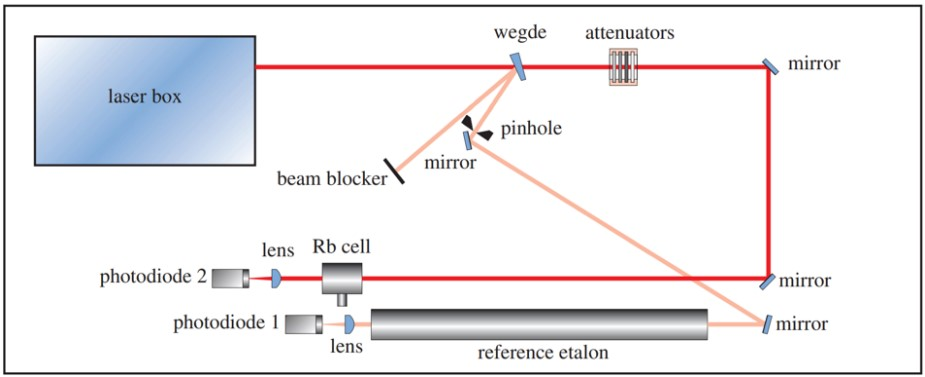
\includegraphics[width = \textwidth]{fig/setup3.jpg}
    \caption{Experimental setup used for linear spectroscopy \cite{lecturenote}}
    \label{fig8}
\end{figure}

\subsection{Measuring Hyperfine Couplings Constants \& Resolution}
\begin{figure}[H]
    \centering
    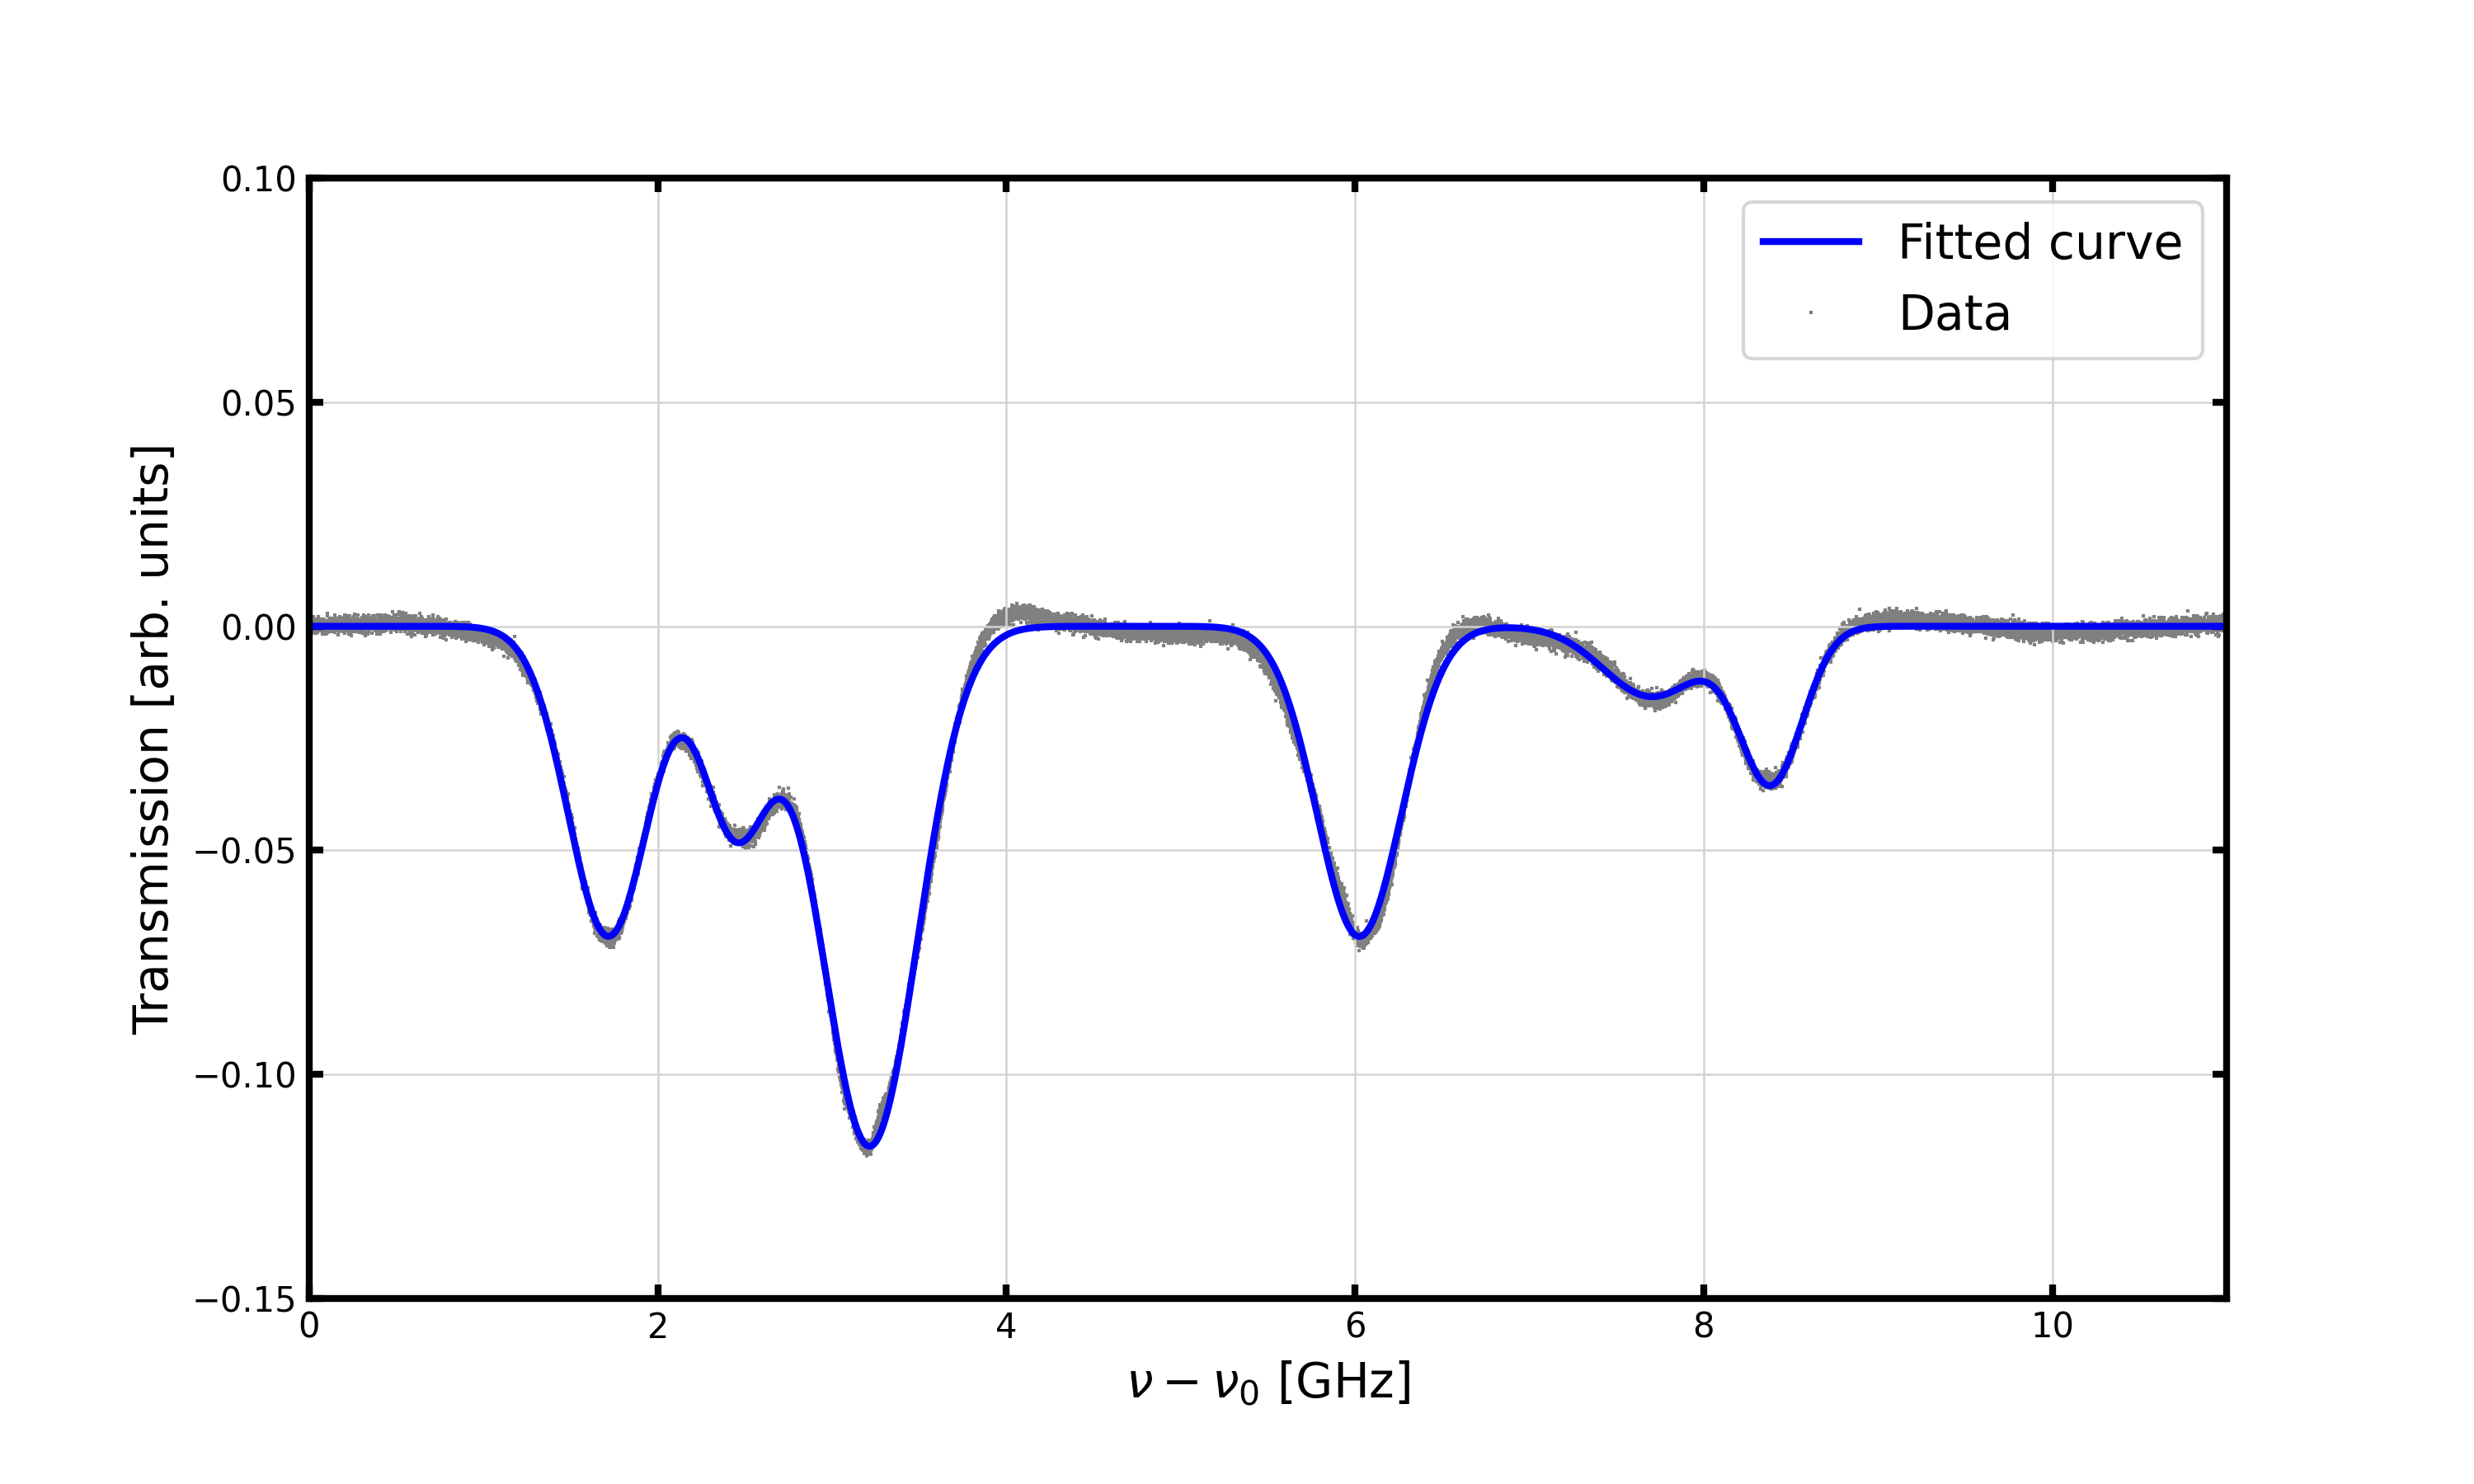
\includegraphics[width = \textwidth]{fig/Experimental_spectrum_backgrundremove.png}
    \caption{Measured absorption spectrum of the 5cm vapor cell}
    \label{fig9}
\end{figure}

Figure \ref{fig9} presents a plot of the measured absorption spectrum of the 5cm vapor cell. To calculate the hyperfine coupling constants, we first fit the data of the spectrum, this is done by using a 5th-degree polynomial for the background and a Gaussian function for the six absorption peaks of the form:
\begin{equation}
    y=\operatorname{A} e^{-\frac{\left(\nu-\nu_0\right)^2}{2 \Delta \nu_{\mathrm{D}}^2}}
    \label{fitting}
\end{equation}

The fitting parameters of the absorption peaks are shown in Table \ref{tab2}. The fitting parameterized the date well, however, there is a clear deviation for the 3rd and 4th lines, this is due to the fact that these lines represent a summation of two Gaussians. 

\begin{table}[H]
    \centering
    \begin{tabular}{c|c|c|c}
         \hline
         \hline
          & A & $\nu_0 [GHz]$ & $\Delta\nu_D [GHz]$   \\
         \hline
         line 1 & $-0.0692 \pm  0.0001$ & $1.7162 \pm 0.0003$ & $0.2303 \pm 0.0004$ \\

         line 2 & $-0.0454 \pm 0.0001 $ & $2.4468 \pm 0.0005$ & $0.1887 \pm 0.0006$ \\   

         line 3 & $-0.1160 \pm 0.0001 $ & $3.2144 \pm 0.0002$ & $0.2748 \pm 0.0003$ \\ 

          line 4 & $-0.0692 \pm 0.0001 $ & $6.0243 \pm 0.0003$ & $0.2416 \pm 0.0004$ \\

          line 5 & $-0.0157 \pm 0.0001 $ & $7.7014 \pm 0.0021$ & $0.2776 \pm 0.0025$ \\

          line 6 & $-0.0348 \pm 0.0001 $ & $8.3853 \pm 0.0008$ & $0.1801 \pm 0.0007$ \\
         
         \hline
    \end{tabular}
    \caption{Fitting parameters of absorbed spectrum}
    \label{tab2}
\end{table}
Following the derivation of energy shifts reported in the previous section, we determine the hyperfine coupling constant of the ground states of both isotopes.   
We compare the relative frequency shifts between the two lines with the energy shifts derived in the previous section. For $^{85}Rb$, this yields:


\begin{equation*}
A_{85}\left(5 S_{1 / 2}\right)=\frac{h}{3} \cdot\left(\nu_0(\text { line } 4)-\nu_0(\text { line } 3)\right)=h \cdot(0.9366 \pm 0.0001) \mathrm{GHz}
\end{equation*}


For $^{87}Rb$, there are two possible line combinations since the hyperfine splitting of the excited state is resolved in the spectrum. Either the frequency difference between lines 1 and 5 or lines 2 and 6 can be used. In our analysis, we take the mean and we get:

\begin{equation*}
A_{87}\left(5 S_{1 / 2}\right)=h \cdot(2.9809 \pm 0.0024) \mathrm{GHz}
\end{equation*}
\\ \\ 
The values given in the literature are \cite{Rb85}\cite{Rb87}:
\begin{equation*}
A_{85}\left(5 S_{1 / 2}\right)=h \cdot 1.011 910 813 0(20) \mathrm{GHz}
\end{equation*}
\begin{equation*}
A_{87}\left(5 S_{1 / 2}\right)=h \cdot3.417 341 305 452 15(5) \mathrm{GHz}
\end{equation*}

We see that we get a discrepancy of around 7.44\% and 12.77\% for $A_{85}(5 S_{1 / 2})$ and $A_{87}(5 S_{1 / 2})$ respectively. 
The deviation could be due to an error of calibration, for example, the assumption that the fringe spacing is constant and not changing, but this is not the case as depicted in Figure \ref{fig5}. Uncertainties in background fitting and errors of oscilloscope measurements can be other sources of the deviation. 

We determine the spectral resolution of each line by calculating $\frac{\Delta\nu}{\nu}$ and taking the mean. The values obtained are reported in Table \ref{tab4}.



\begin{table}[H] \centering  \begin{tabular}{c|c} 
\hline
\hline 
& Resolution R  $ \times 10^{-6} [GHz]$ \\
\hline 
line 1 & $1.44 \pm 0.03$ \\
line 2 & $1.18 \pm 0.04$ \\
line 3 & $1.72 \pm 0.02$ \\
line 4 & $1.51 \pm 0.02$ \\
line 5 & $1.73 \pm 0.16$ \\
line 6 & $1.13 \pm 0.05$ \\
\hline 
\end{tabular}
\caption{Lines spectral resolution from linear spectroscopy}
\label{tab4} 
\end{table}

Calculating the mean of spectral resolution yields:
\begin{equation*}
R = (1.45 \pm 0.02) \times 10^{-6}
\end{equation*}
This resolution is high enough to observe the ground state splitting of both isotopes and the splitting of the excited state of $^{87}Rb$, but it is not possible to separate the excited state splitting with this resolution. 

\subsection{FWHM \& Doppler Broadening}
$nu_{FWHM}$ can be solved from equation \ref{fitting} as:
\begin{equation*}
       \operatorname{A} e^{-\frac{\left(\nu-\nu_0\right)^2}{2 \Delta \nu_{\mathrm{D}}^2}} = \frac{A}{2}
\end{equation*}
which yields:
\begin{equation*}
\delta \nu_{\mathrm{FWHM}}=2 \sqrt{2 \ln 2} \Delta \nu_{\mathrm{D}}
\end{equation*}
 Using this equation and the Doppler width values reported in Table \ref{tab2}, we get the values of FWHM shown in Table \ref{tab5}.

 \begin{table}[H] \centering  \begin{tabular}{c|c|c} 
\hline
\hline 
& $\delta \nu_{FWHM} [MHz]$ &  Isotope \\
\hline 
line 1 & $542.3 \pm 1.1$ & $^{87}Rb$ \\
line 2 & $444.3 \pm 1.5$ & $^{87}Rb$ \\
line 3 & $647.2 \pm 0.7$ & $^{85}Rb$ \\
line 4 & $569.0 \pm 0.9$ & $^{85}Rb$ \\
line 5 & $653.8 \pm 6.0$ & $^{87}Rb$ \\
line 6 & $424.2 \pm 1.7$ & $^{87}Rb$ \\

\hline 
\end{tabular}
\caption{Values of FWHM from linear spectroscopy}
\label{tab5} 
\end{table}

Now to make a comparison with the theoretical values, we first calculate the theoretical values using the formula:
\begin{equation*}
\Delta \nu_{\mathrm{D}}=\nu_0 \sqrt{\frac{k_{\mathrm{B}} T}{m c^2}}
\end{equation*}
At room temperature of 300K and with atomic mass values from \cite{Rb85}\cite{Rb87}. 

This yields for the two isotopes:

\begin{table}[h] \centering

\begin{tabular}{c|c|c} 
\hline
\hline
Isotope & $\Delta \nu_{\mathrm{D}} [MHz]$ & $\delta \nu_{\mathrm{FWHM}} [MHz]$ \\
\hline${ }^{85} \mathrm{Rb}$ & 215.595 & 507.682 \\
${ }^{87} \mathrm{Rb}$ & 213.103 & 501.815\\
\hline
\end{tabular}
\caption{Theoretical Values of FWHM}
\label{tab6}
\end{table}

By comparing the mean values in Table \ref{tab5} and the theoretical values in Table \ref{tab6}. We see mean values of $\delta \nu_{\mathrm{FWHM}} $ = ($516.15 \pm 2.58$) and $\delta \nu_{\mathrm{FWHM}} $ = ($608.1 \pm 0.1$) with discrepancies of $2.85 \%$ and $19.78 \%$ for $^{87} \mathrm{Rb}$ and $^{85} \mathrm{Rb}$ respectively. The mean value for $\delta \nu_{\mathrm{FWHM}} $ for $^{87} \mathrm{Rb}$ almost shows an agreement with what is expected with a slight deviation that could be due to the assumption of constant fringe spacing. However, there is a significant deviation for the case of $^{85} \mathrm{Rb}$ which is due to the inability of linear spectroscopy to resolve some peaks, the fit overestimates the width of the peaks since a single Gaussian peak is fitted to a superposition of two peaks. 

\subsection{Verifiying Lambert-Beer Law}

We measure and record the transmission spectrum for different vapor cells of different lengths (2 cm, 5 cm, and 7 cm). Then, we fit the spectrum with a polynomial background and six Gaussian functions. The transmission spectrum for different vapor cells is shown in Figure \ref{fig10}. 

To verify the law, we plot the amplitude of peaks against the length of vapor cells in Figure \ref{fig11}. As seen from the figure, the absorption increases for longer cells, which is the case for all cases. Thus, the law is verified. However, there are significant deviations from the linear correlation which is due to the experimental setup. For example, cells may not be mounted exactly parallel to the beamline, this increases the length of a cell and increases the fraction of beam reflected by the glass panes in the vapor cell. Also, a cell may have scratches in its glass panes which affects its absorption, making it stronger.  
One may increase the reliability of the measurement by increasing the data points, carefully adjusting the alignment of the cells, and also with a good choice of cells. 
\begin{figure}[H]
    \centering
    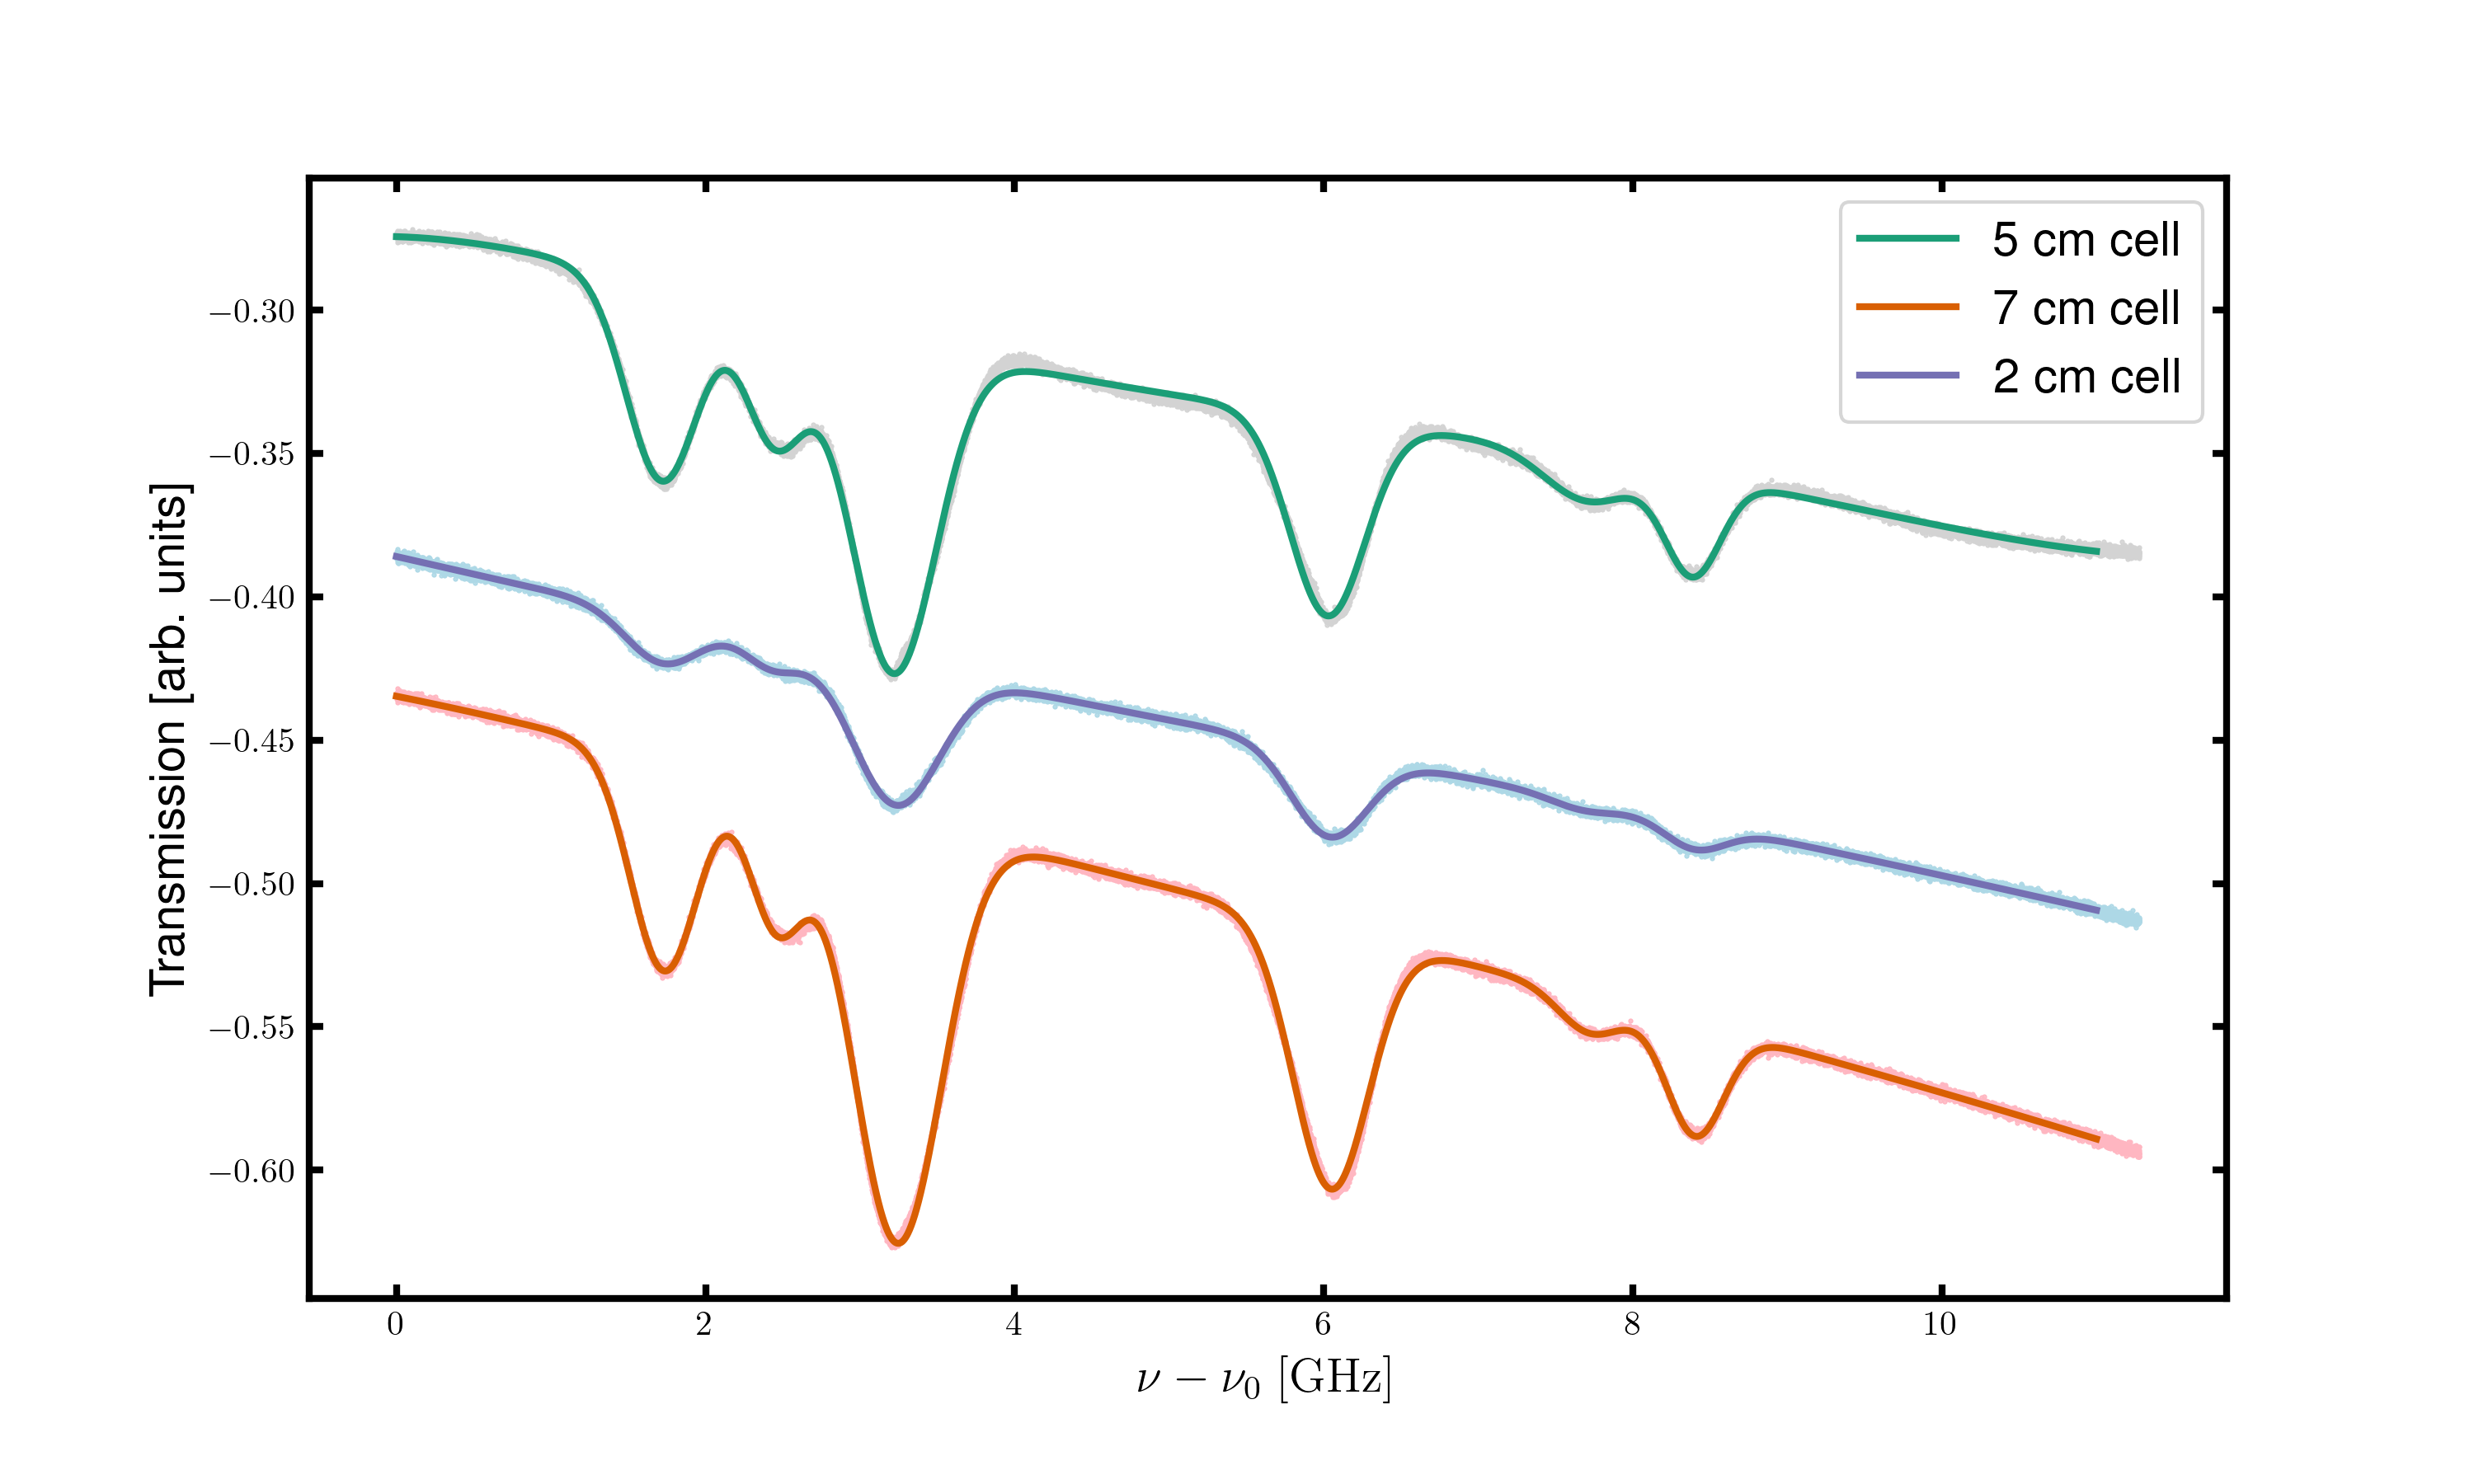
\includegraphics[width = \textwidth]{fig/All_spectra.png}
    \caption{Measured absorption spectrum of different vapor cells with different lengths}
    \label{fig10}
\end{figure}


\begin{figure}[H]
    \centering
    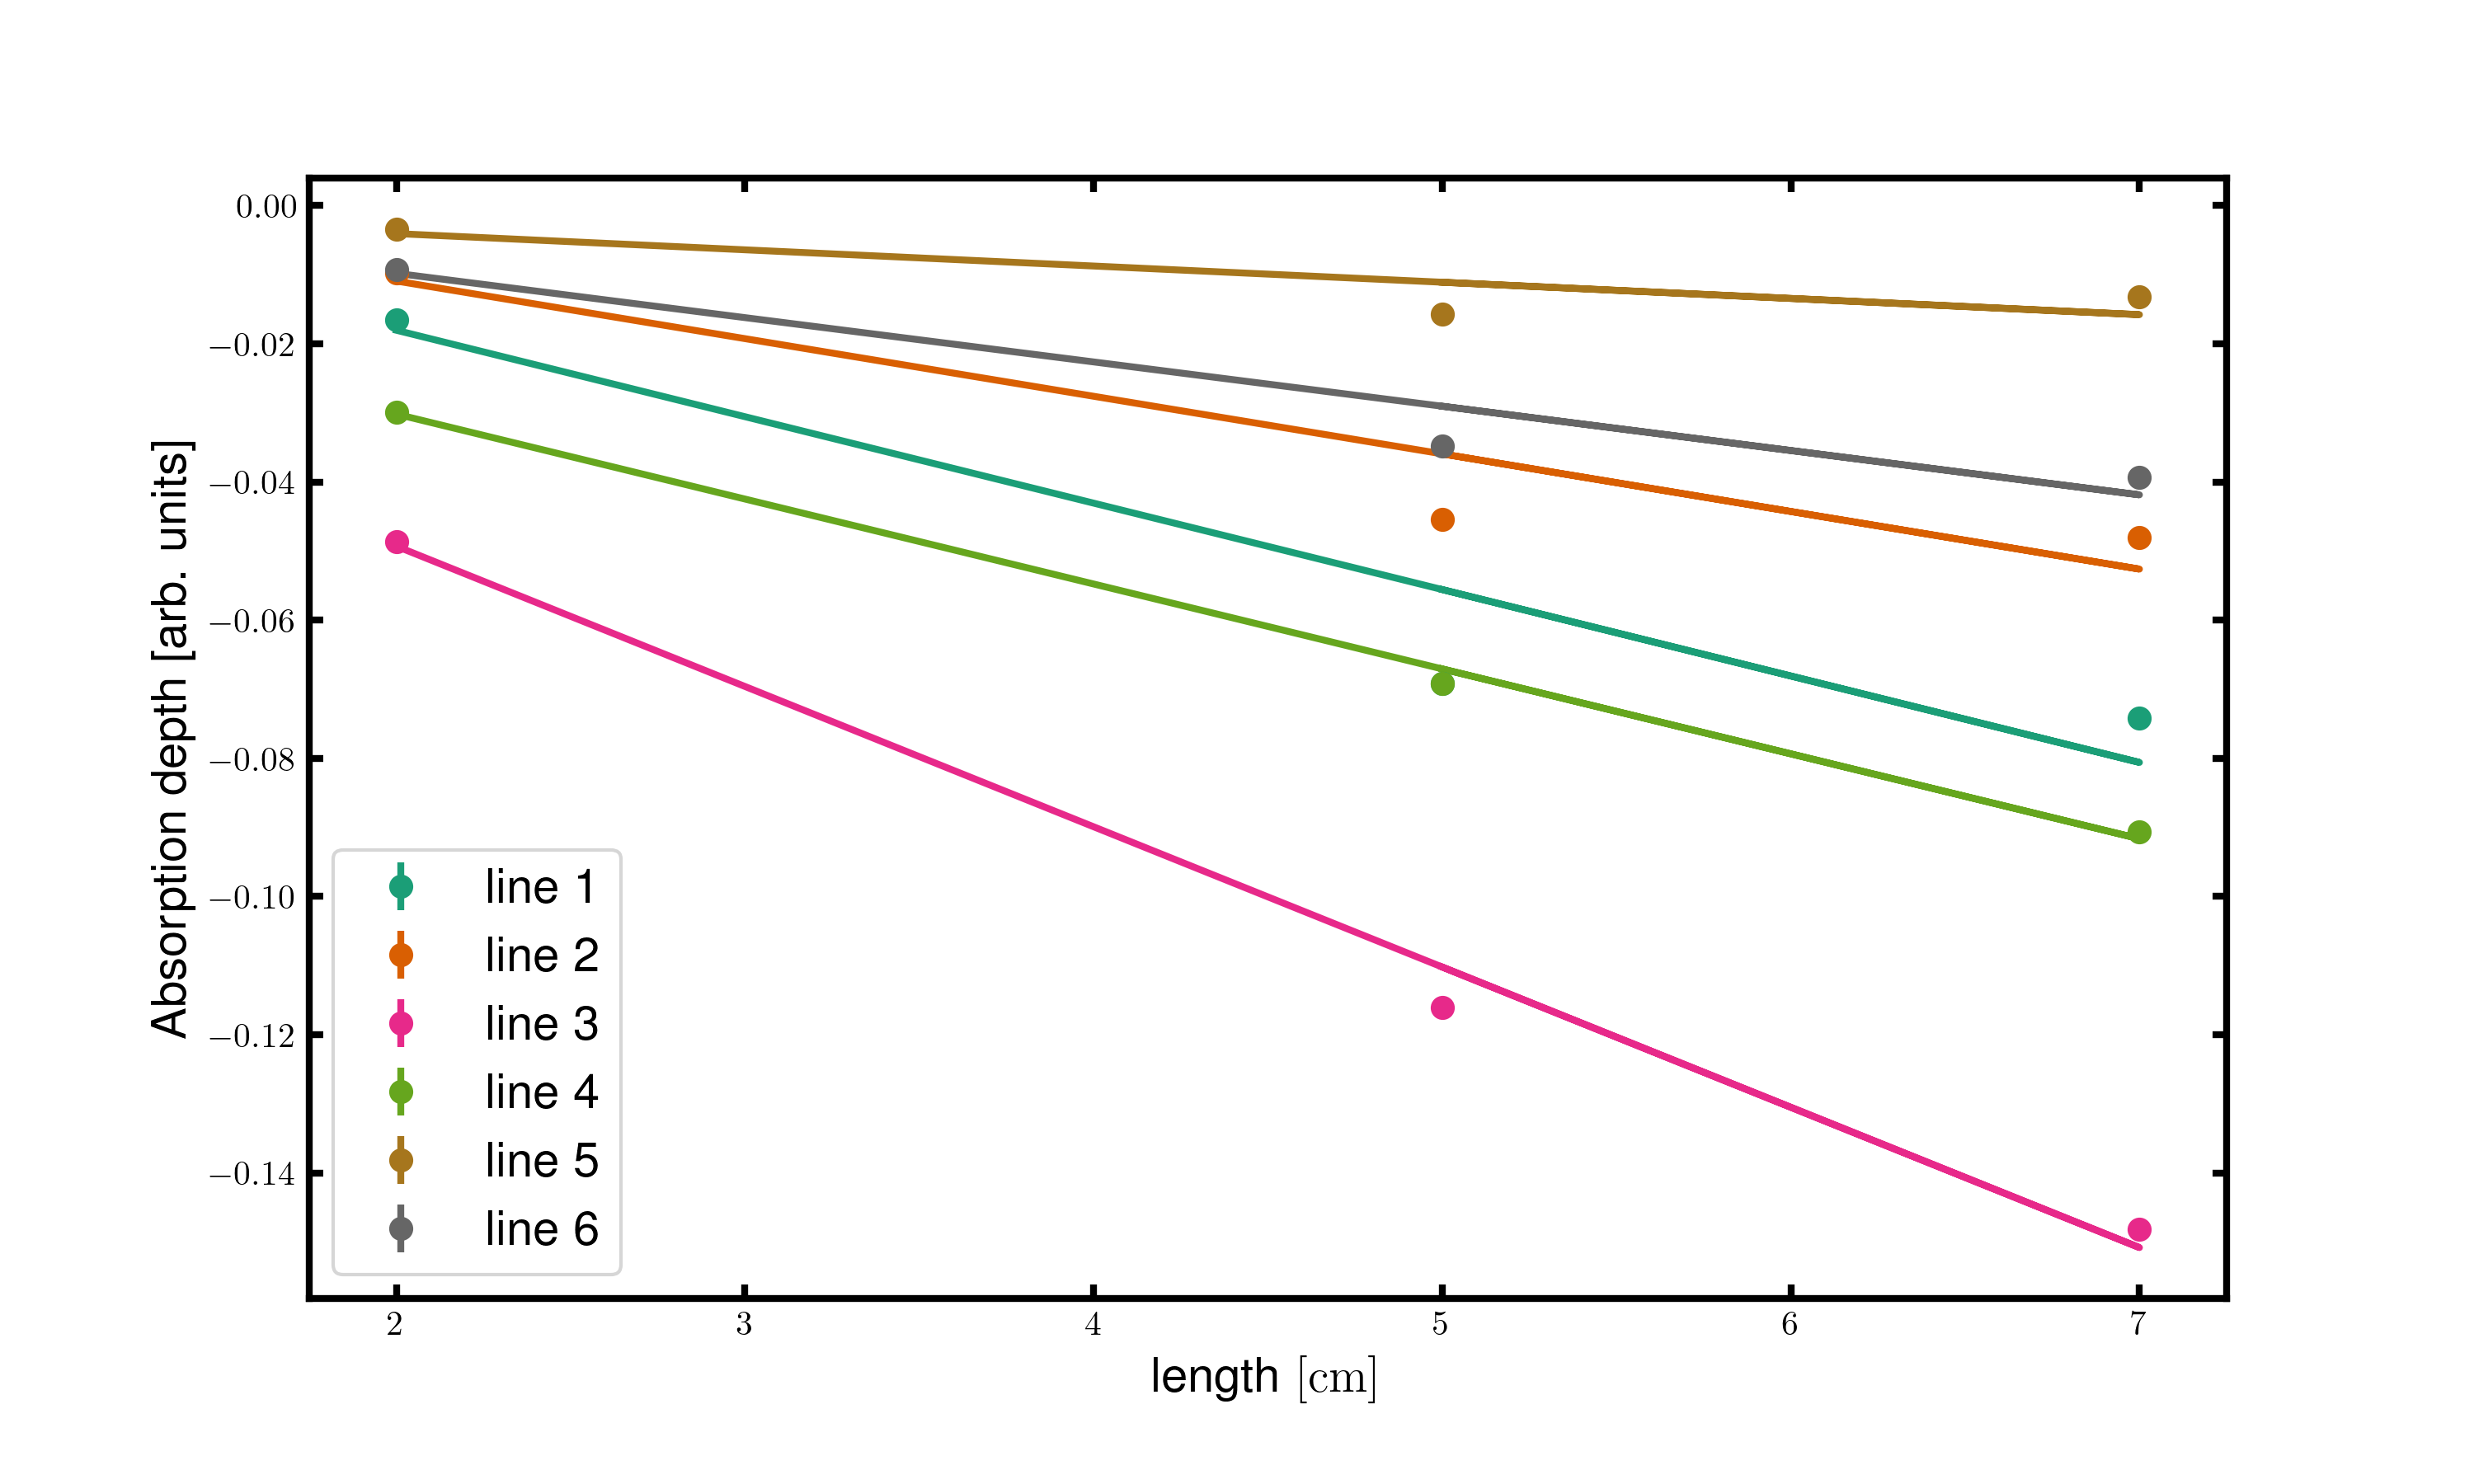
\includegraphics[width = \textwidth]{fig/Lambeert_Beer.png}
    \caption{Dependence of vapor absorption on the length of the vapor cell}
    \label{fig11}
\end{figure}

\section{Non-Linear Spectroscopy}

In this part of the experiment, we use non-linear spectroscopy to resolve the hyperfine structure of $^{85}Rb$ and $^{87}Rb$ as it is a Doppler-free type of spectroscopy. We again determine the main characteristics of the hyperfine structures such as the hyperfine constants, examine the spectral resolution, and also determine the saturation intensity of Rubidium.


\subsection{Experimental Setup}

\begin{figure}[H]
    \centering
    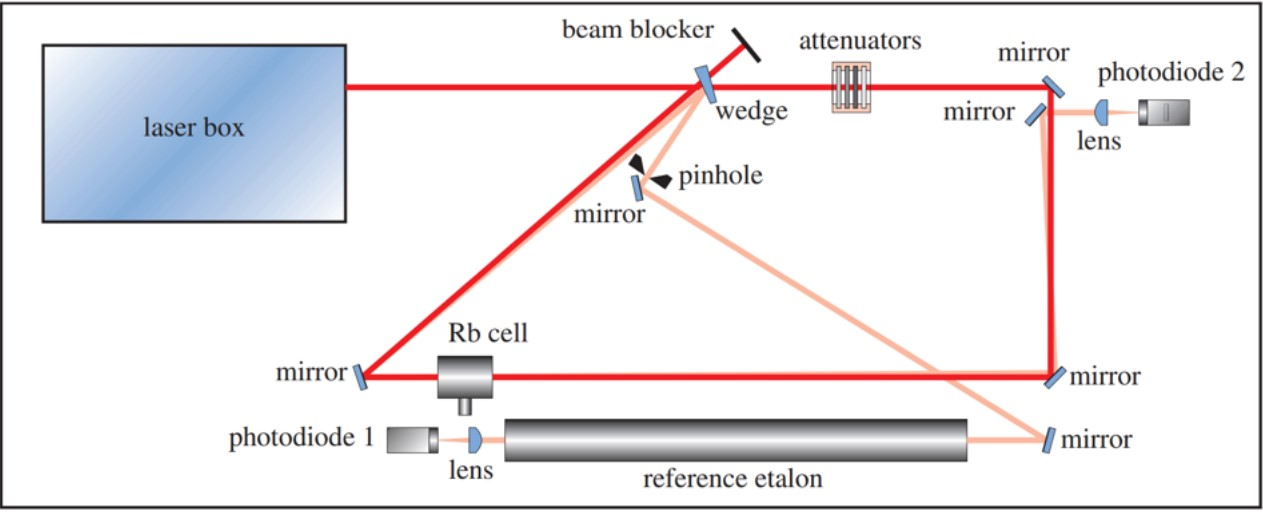
\includegraphics[width = \textwidth]{fig/setup4.jpg}
    \caption{Expermiental setup of non-linear spectroscopy \cite{lecturenote}}
    \label{fig12}
\end{figure}

To measure the Doppler-free absorption spectrum of Rubidium, a saturated absorption spectroscopy is needed. The idea of a saturation setup is the following, a pump beam 
is used to saturate the excited states of both rubidium isotopes, and another weaker beam from the same laser is used to probe the spectrum. Here, the strong transmitted beam used in the linear spectroscopy part is utilized to be the pump beam and blocked after passing a 7cm vapor cell using a beam blocker. Also, we remove the blocking of the third laser beam in \ref{fig8} and guide this beam to pass the cell in a direction opposite to the pump beam. This is done to achieve a maximum overlap in the vapor cell for interaction with the same atoms. As a result, the paths of both beams is maximized and the incident angle with respect to the vapor cell is minimized. This second beam works now as a probe beam and is focused on a photodiode to measure the transmitted power after passing the vapor cell. Figure \ref{fig12} shows the experimental setup used for non-linear spectroscopy. 

\subsection{Measuring Hyperfine Couplings Constants \& Res-
olution}

Using the same analysis in the linear spectroscopy part, we plot the resulting spectrum in Figure \ref{fig13}. Now, the dips corresponding to the substructure of the hyperfine structure of Rubidium can be seen. We neglect the central dips of the central lines for further analysis since they are cross-over peaks. 



\begin{figure}[H]
    \centering
    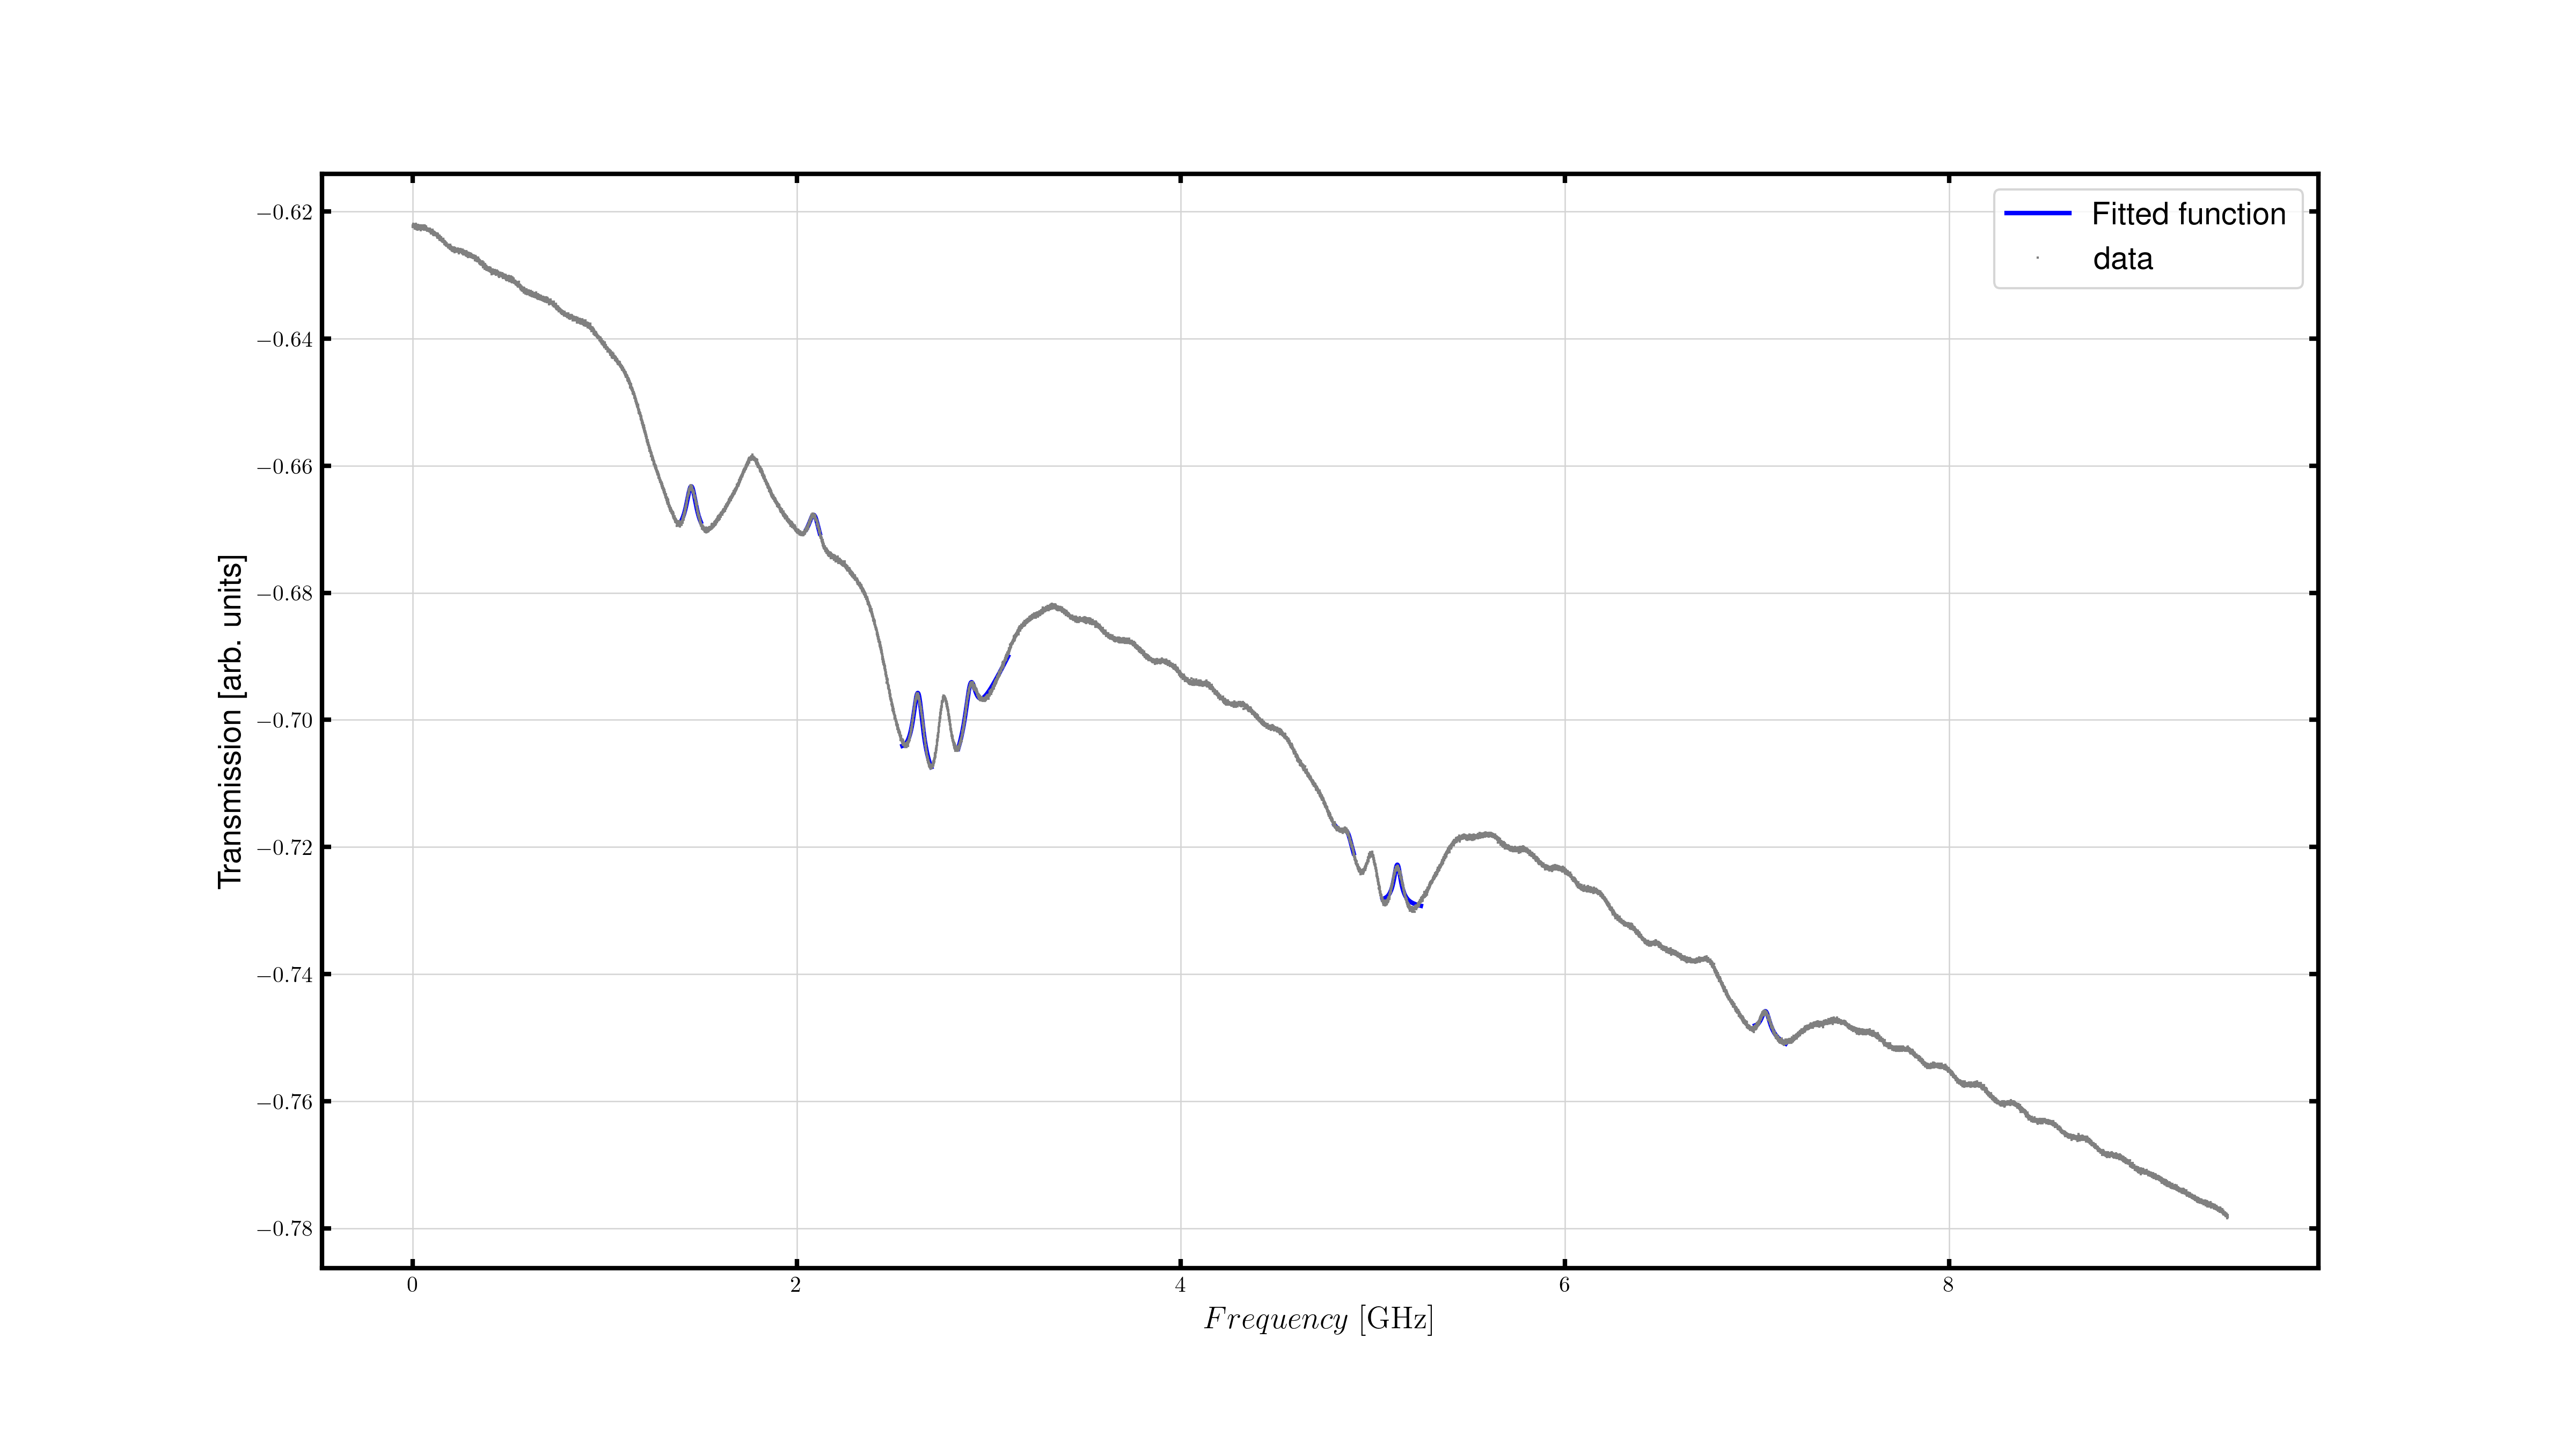
\includegraphics[width = \textwidth]{fig/dip_analysis.png}
    \caption{Absorption spectrum of Rubidium using non-linear spectroscopy}
    \label{fig13}
\end{figure}

We fit the Doppler-free peaks using a Lorentzian line profile with an additional linear background of the form:
\begin{equation}
f(\nu)=A \cdot \frac{\left(\frac{\text { FWHM }}{2}\right)^2}{\left(\nu-\nu_0\right)^2+\left(\frac{\mathrm{FWHM}}{2}\right)^2}+B \cdot \nu+C
\label{spectrumfit}
\end{equation}

where $\nu_0$ is the resonance frequency of the two-level system, FWHM is the Full Width of Half Maximum and A, B, and C are the fitting parameters.

Similar to the linear spectroscopy part, we calculate the hyperfine coupling constants from the difference between the position of the dips. For $^{85}Rb$, we get:

\begin{equation*}
A_{85}\left(5 S_{1 / 2}\right)=h \cdot(3.3318 \pm 0.0007) \mathrm{GHz}
\end{equation*}

\begin{equation*}
A_{85}\left(5 P_{1 / 2}\right)=h \cdot(0.3274 \pm 0.0001) \mathrm{GHz}
\end{equation*}

For $^{87}Rb$, we get:

\begin{equation*}
A_{87}\left(5 S_{1 / 2}\right)=h \cdot(10.2961 \pm 0.4000) \mathrm{GHz}
\end{equation*}

\begin{equation*}
A_{87}\left(5 P_{1 / 2}\right)=h \cdot(1.2400 \pm 0.0002) \mathrm{GHz}
\end{equation*}

Now, we compare these values to the literature values presented in \cite{Rb85}\cite{Rb87}, given as:

\begin{equation*}
A_{85}\left(5 S_{1 / 2}\right)=h \cdot 1.011 910 813 0(20)  \mathrm{GHz}
\end{equation*}


\begin{equation*}
A_{85}\left(5 P_{1 / 2}\right)=h \cdot  0.120 527(56) \mathrm{GHz}
\end{equation*}


\begin{equation*}
A_{87}\left(5 S_{1 / 2}\right)=h \cdot3.417 341 305 452 15(5) \mathrm{GHz}
\end{equation*}

\begin{equation*}
A_{87}\left(5 P_{1 / 2}\right)=h \cdot 0.407 25(63) \mathrm{GHz}
\end{equation*}

Apparently, we had a problem with the calibration and values got multiplied by around a factor of 3. Therefore, we divide all the resulting values by a factor of 3 and calculate the errors. As a result, we get errors of $9.75\%$, $9.45\%$, $0.43\%$, and $1.49\%$ for $A_{85}\left(5 S_{1 / 2}\right)$, 
$A_{85}\left(5 P_{1 / 2}\right)$, 
$A_{87}\left(5 S_{1 / 2}\right)$, and $A_{87}\left(5 P_{1 / 2}\right)$, respectively. Possible errors of the linear spectroscopy hold here as well. Also, the increased multiplied factor is not known accurately, and hence we do not get the exact errors. 

The mean spectral resolution obtained is calculated using the same approach in the linear spectroscopy part for a laser frequency of 377.57 THz, we get:
\begin{equation*}
    R = (1.69 \pm 2.4) \times 10^{-8}
\end{equation*}
This is two orders lower than the value obtained in the linear spectroscopy part, which is expected since the resolution of linear spectroscopy is limited by Doppler broadening, which can also be visible by comparing the two spectra as some lines are not visible in the linear spectroscopy spectrum. 

\subsection{Saturation Power}
In this part of the experiment, we determine the the intensity of laser needed to saturate the Rubudium. This is done by 
examining how the amplitude A and line width $\nu$ of the dip corresponding to the 5S1/2(F = 2) $\xrightarrow{}$  5P1/2(F = 1) hyperfine component of $^{87}Rb$, which appears as the leftmost feature in the previous absorption spectrum, vary with different levels of pump laser power and attenuation.

We use different attenuators of different transmission coefficients (0.037, 0.321, 0.512, and 0.955) and their combinations. We record the FPI spectrum and convert it to a frequency spectrum similar to the linear spectroscopy part.

The output power of the laser beam is calculated by multiplying its power with the transmission coefficient used. We fit dips using the same Lorentzian function \ref{spectrumfit}. We present the resulting plots in Figure \ref{fig14}.  We also show the relation between  Laser power on amplitude and line width in Figure \ref{fig15}.

\begin{figure}[H]
    \centering
    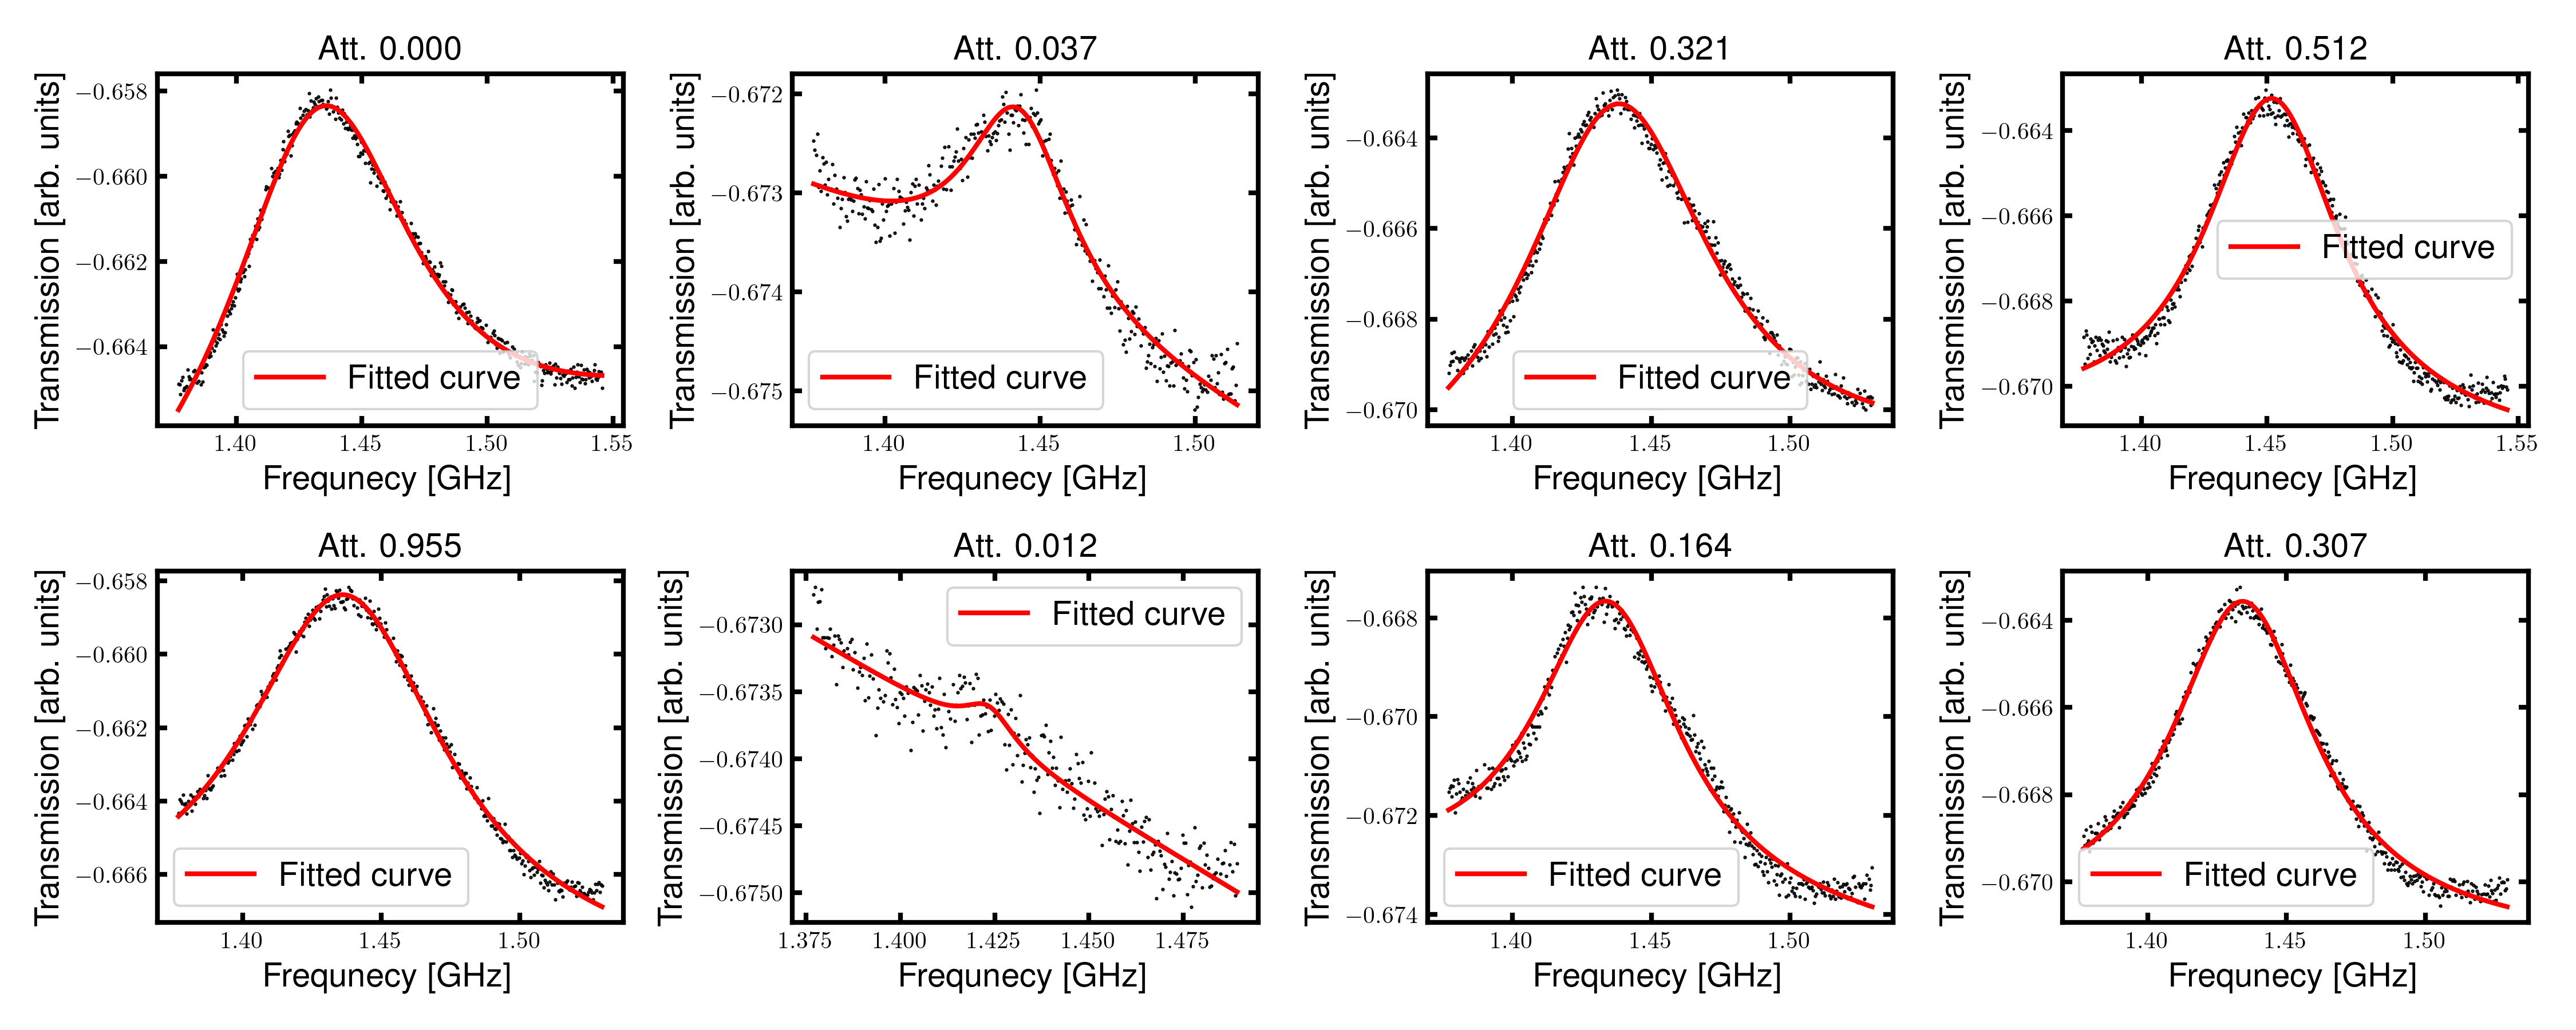
\includegraphics[width = \textwidth]{fig/saturation_fit.png}
    \caption{Fitting of the 5S1/2(F = 2) $\xrightarrow{}$ 5P1/2(F = 1) hyperfine component of $^{85}Rb$ for different attenuations}
    \label{fig14}
\end{figure}

\begin{table}[H]
    \centering
    \begin{tabular}{c|ccc}
Attenuator & FWHM &  $\nu_0$ & A   \\
\hline
$0.0000$ & $0.0920 \pm 0.0012$& $1.4337 \pm 0.0002$& $0.0100 \pm 0.0001$ \\
$0.0370$ & $0.0418 \pm 0.0015$& $1.4429 \pm 0.0003$& $0.0020 \pm 0.0000$ \\ 
$0.3210$ & $0.0823 \pm 0.0013$& $1.4377 \pm 0.0002$& $0.0086 \pm 0.0001$ \\ 
$0.5120$ & $0.0656 \pm 0.0010$& $1.4520 \pm 0.0002$& $0.0078 \pm 0.0001$ \\ 
$0.9550$ & $0.0882 \pm 0.0011$& $1.4366 \pm 0.0002$& $0.0098 \pm 0.0001$ \\ 
$0.0119$ & $0.0167 \pm 0.0045$& $1.4235 \pm 0.0012$& $0.0003 \pm 0.0000$ \\ 
$0.1644$ & $0.0638 \pm 0.0014$& $1.4341 \pm 0.0003$& $0.0061 \pm 0.0001$ \\ 
$0.3066$ & $0.0629 \pm 0.0009$& $1.4343 \pm 0.0002$& $0.0075 \pm 0.0001$   
    \end{tabular}
    \caption{Fitting parameters for the 5S1/2(F = 2) $\xrightarrow{}$ 5P1/2(F = 1) hyperfine component of $^{85}Rb$ for different attenuations}
    \label{tab7}
\end{table}

\begin{figure}[H]
    \centering
    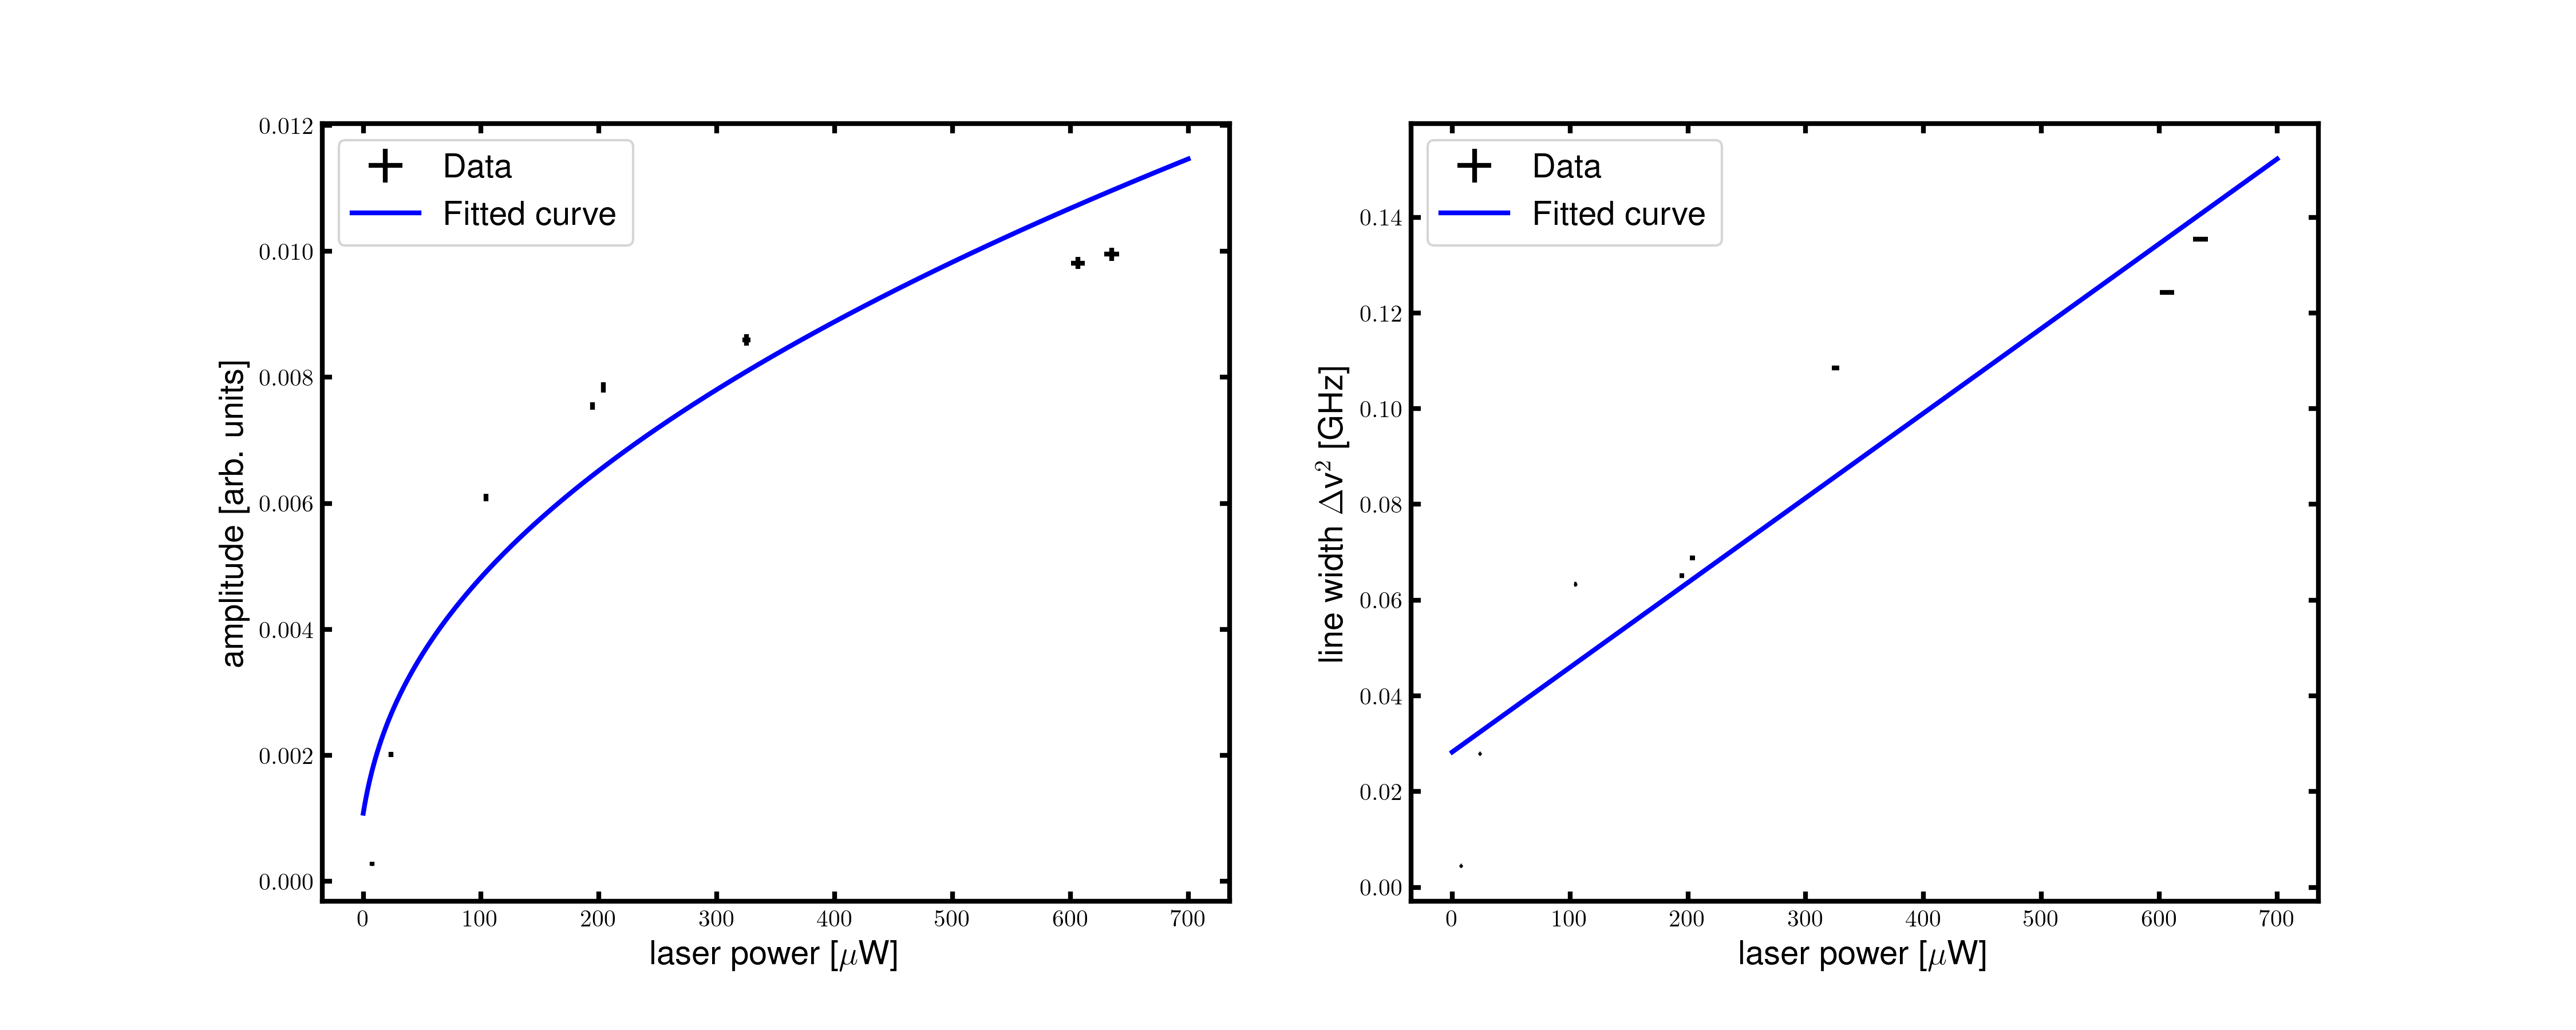
\includegraphics[width = \textwidth]{fig/saturation-power.png}
    \caption{Dependence of Laser power on amplitude (left) and line (right ) of the 5S1/2(F = 2) $\xrightarrow{}$ 5P1/2(F = 1) hyperfine component of $^{85}Rb$ for different attenuations}
    \label{fig15}
\end{figure}

As a result, we get a saturation power and saturation line width of:
% \begin{equation*}
%     P_{sat} = $11.7278 \pm 3.006$
% \end{equation*}

% \begin{equation*}
%     P_{sat_linewidth} = $12.633 \pm 0.831$
% \end{equation*}

Possible errors of the obtained values may include having only part of the beam interacting with the vapor cell due to misalignment in the setup and also due to reduction of the beam because of beam splitting.

\section{Error Discussion}

\subsection{Diode laser characteristics}
Possible errors in this part of the experiment include variations in laser intensity, background noise, oscilloscope errors, and imperfections in the lenses and used elements in the setup. 

\subsection{The Fabry-Perot interferometer}
Errors that contribute to a deviation of the obtained value of FBI finesse include a misalignment of the FBI in the beamline, scratches on the surface of the mirrors, and also having disturbances in the periodicity of transmission peaks. 

\subsection{Linear Spectroscopy}
Here we had a problem with the obtained values of the hyperfine coupling constant which was due to the error of calibrating the frequencies. Also, the fitting is due to peaks being unresolved. In verifying Lambert-Beer law, we had a deviation from the linear correlation which is due to the low number of data points used. Also, oscilloscope errors, misalignment, and imperfections of parts of the setup play a key role. 

\subsection{Non-Linear Spectroscopy}
In addition to all the mentioned errors, a possible misalignment in the overlay of the problem and pump and a deviation in the incident angle under which the beam enters the vapor cell can affect the accuracy of the data. 

\section{Conclusion}
All in all, we investigate the main characteristics of a diode laser, its linear behavior (injected current vs. output power) along with calculating its slope and quantum efficiency. We get a threshold current $I_{thr} = 54 \pm 1 \mathrm{mA}$ and a slope efficiency $a= 10.41 \pm 0.08 \mathrm{\dfrac{W}{A}}$. \\
Then, we moved to to investigate the properties of the FPI. We used the FPI to set a reference for calibration frequencies and we got a calibration constant $c_{calibration} = 479.94 \pm 0.242$. \\

Furthermore, we conduct a linear spectroscopy to obtain the absorption spectrum of both Rubidium isotopes. We calculated the hyperfine coupling constants of the transitions of both isotopes, we obtained 
\begin{equation*}
    A_{85}\left(5 S_{1 / 2}\right)=\frac{h}{3} \cdot\left(\nu_0(\text { line } 4)-\nu_0(\text { line } 3)\right)=h \cdot(0.9366 \pm 0.0001) \mathrm{GHz}
\end{equation*}

\begin{equation*}
    A_{87}\left(5 S_{1 / 2}\right)=h \cdot(2.9809 \pm 0.0024) \mathrm{GHz}
\end{equation*}
\\
Then we moved to conducting non-linear spectroscopy to eliminate the Doppler-broadening effect and resolve the hidden lines. We do the same analysis and get hyperfine coupling constants of 
\begin{equation*}
    A_{85}\left(5 S_{1 / 2}\right)=h \cdot(3.3318 \pm 0.0007) \mathrm{GHz}
\end{equation*}
\begin{equation*}
    A_{85}\left(5 P_{1 / 2}\right)=h \cdot(0.3274 \pm 0.0001) \mathrm{GHz}
\end{equation*} 
\begin{equation*}
 A_{87}\left(5 S_{1 / 2}\right)=h \cdot(10.2961 \pm 0.4000) \mathrm{GHz}   
\end{equation*}
\begin{equation*}
 A_{87}\left(5 P_{1 / 2}\right)=h \cdot(1.2400 \pm 0.0002) \mathrm{GHz}    
\end{equation*}
 \\ 
Finally, we investigate the effect of laser intensity on saturation drawing correlations. \\
Multiple deviations of the obtained values are realized due to multiple possible sources of errors that are fully discussed in section 6.
\printbibliography



\end{document}